%%
%% This is file `squelette-rr.tex',
%% generated with the docstrip utility.
%%
%% The original source files were:
%%
%% RR.dtx  (with options: `sample')
%% *******************************************************************
%% Copyright (C) 1997-1999 INRIA/MIAOU
%% 
\documentclass{article}

%\usepackage{a4}
\usepackage{amsmath}
%\usepackage{french}
\usepackage{rotating}
%\usepackage{epsfig}
%\usepackage{graphicx}
\usepackage{float}
\usepackage{amssymb}
\usepackage{array}

\usepackage{RR}
\usepackage{hyperref}
\usepackage{french} % optionnel
%%\usepackage[frenchb]{babel} % optionnel
%%
\RRdate{Novembre 2002} %  date de publication du rapport
%%
\RRauthor{
J. Fr\'ed\'eric Bonnans 
\thanks[sydoco]{Projet Sydoco} 
\and % \and entre chaque auteur s'il y en a plusieurs
Jean-Marc Cognet
\thanks[edf-mathfi]{EDF Recherche et D\'eveloppement, 
1 avenue du G\'en\'eral de Gaulle, BP 408, 92141 Clamart. 
Travail effectu\'e dans le cadre d'un Post-Doctorat Industriel 
au sein du projet Mathfi}
\and
Sophie Volle
\thanks[raise-partner-mathfi-sydoco]{Raise Partner, 
3 Chemin de ronde, 38000 Grenoble. Travail effectu\'e dans le cadre 
d'un poste d'accueil des projets Mathfi et Sydoco}
}
%%
\authorhead{J.F. Bonnans, J.-M. Cognet et S. Volle} 
% Ceci apparait sur chaque page paire.
%%
\RRtitle{Estimation de la volatilit\'e locale d'actifs financiers 
par une m\'ethode d'inversion num\'erique} % titre francais
%%
\RRetitle{Estimation of the local volatility of financial assets 
by a numerical inversion method} % english title
%%
\titlehead{Estimation de la volatilit\'e locale} 
%titre court, sur toutes les pages.
%%
%%\RRnote{This is a note}
%%\RRnote{This is a second note}
%%
\RRresume{
Nous nous int\'eressons \`a un probl\`eme de calibration 
rencontr\'e en finance qui consiste \`a identifier la 
volatilit\'e locale \`a partir de prix d'options observ\'es sur 
le march\'e. Nous formulons le probl\`eme sous la forme d'un 
probl\`eme inverse. Le probl\`eme direct (pricing), qui consiste 
\`a calculer les prix d'options en r\'esolvant l'\'equation aux 
d\'eriv\'ees partielles de Dupire, est r\'esolu par diff\'erences 
finies. Le probl\`eme inverse (calibration) revient ensuite \`a 
r\'esoudre un probl\`eme d'optimisation dans lequel il s'agit de 
d\'eterminer la volatilit\'e optimale telle que les prix calcul\'es 
avec cette volatilit\'e soit le plus proche possible des prix 
observ\'es sur le march\'e. Ce probl\`eme inverse mal pos\'e est 
r\'egularis\'e en param\'etrant la volatilit\'e par des splines 
bicubiques et en adoptant une approche multi\'echelle. De plus, 
nous utilisons l'algorithme de Quasi-Newton (avec ou sans bornes) 
pour r\'esoudre le probl\`eme d'optimisation. Notre algorithme de 
calibration est test\'e sur des donn\'es synth\'etiques (simul\'ees 
par notre mod\`ele) et sur des donn\'ees r\'eelles du march\'e.
}
%%
\RRabstract{
We consider a problem arising in finance that consists 
in identifying the local volatility from option prices provided by 
the market. The problem is formulated as an inverse problem. The 
direct problem (pricing), which consists in computing option 
prices by solving Dupire's partial differential equation, is 
solved by finite differences. Then, the inverse problem 
(calibration) consists in solving an optimization problem where 
we have to determine the optimal volatility such that the prices 
computed with this volatility are as close as possible to the 
prices given by the market. This ill-posed inverse problem is 
regularized by parameterizing the volatility using bicubic 
splines and by employing a multiscale approach. Moreover, we use 
the Quasi-Newton algorithm (with or without bounds) to solve 
the optimization problem. Our algorithm of calibration is tested 
on synthetic data (simulated with our model) and on real data 
provided by the market.
}
%%
\RRmotcle{finance, calibration, EDP de Dupire, diff\'erences finies, 
probl\`eme inverse, optimisation}
%%
\RRkeyword{finance, calibration, Dupire's PDE, finite differences, 
inverse problem, optimization}
%% \RRprojet{Miaou} % cas d'un seul projet
%%
%%\RRprojets{Miaou et Op�ra} % cas de 2 projets.
\RRprojets{Mathfi et Sydoco} % cas de 2 projets.
%%
\RRtheme{4} % cas d'un seul theme
%%\RRtheme{43} % cas de 2 themes
%%
%% \URLorraine % pour ceux qui sont � l'est
%% \URRennes  % pour ceux qui sont � l'ouest
%% \URRhoneAlpes % pour ceux qui sont dans les montagnes
\URRocq % pour ceux qui sont au centre de la France
%% \URFuturs % pour ceux qui sont dans le virtuel
%% \URSophia % pour ceux qui sont au Sud.
%%

\newcommand{\nc}{\newcommand}
\nc{\rnc}{\renewcommand}

\nc{\draft}{true}
\nc{\draftfig}{false}

\nc{\dsp}{\displaystyle}

\newtheorem{Rem}{Remarque}
\newtheorem{lemme}{Lemme}
\newtheorem{defi}{D\'efinition}
\newtheorem{theo}{Th\'eor\`eme}
\newtheorem{corr}{Corrolaire}

\newcommand {\bsigma}{\bar{\sigma}}
\newcommand {\vertBox}[1]{\begin{sideways}\fbox{#1}\end{sideways}}

\newcommand{\noi}{\noindent}
\newcommand{\bs}{\bigskip}
\newcommand{\ms}{\medskip}
\newcommand{\debdem}{{\bf D\'emonstration.}\quad}
\newcommand\findem{\hfill{$\blacksquare$}\medskip}

% \newcommand{\debdem}{\begin{proof}} \def\findem{\end{proof}}

\newcommand{\refeq}[1]{(\ref{#1})}
%\newcommand{\eqref}[1]{(\ref{#1})}

\def\sharpo{{ }}

\def\1B{{\bf  1}}
\def\argmin{\mathop{\rm argmin}}
\def\argmax{\mathop{\rm argmax}}
\def\dw{\mathop{\delta w}}

\def\cl{\mathop{\rm cl}}
\def\conv{\mathop{\rm conv}}
\def\diag{\mathop{\rm diag}}
\def\dist{\mathop{\rm dist}}
\def\dom{\mathop{{\rm dom}}}
\def\supp{\mathop{\rm supp}}
\def\val{\mathop{\rm val}}
\def\var{\mathop{\rm var}}
\def\epi{\mathop{\text{\'epi}}}
\def\isom{\mathop{\rm Isom}}
\def\inv{\mathop{\rm inv}}
\def\intt{\mathop{\rm int}}
\def\Ker{\mathop{\rm Ker}}

\def\Inf{\mathop{\rm Inf}}
\def\Min{\mathop{\rm Min}}
\def\Max{\mathop{\rm Max}}


\def\rar{\rightarrow}
\def\trace{\mbox{trace}}

\newcommand\be{\begin{equation}}
\newcommand\ee{\end{equation}}
\newcommand\ba{\begin{array}}
\newcommand\ea{\end{array}}
\def\disp{\displaystyle}
% \def\cR{I\hspace{-1mm}R}
\def\cZ{\mathbb{Z}}

\newcommand{\cE}{I\!\!E}
\newcommand{\cR}{I\!\! R}
\newcommand{\cRbar}{\bar {I\!\! R}}
\newcommand{\cN}{I\!\!N}

\def\Om{{\Omega}}
\def\om{{\omega}}
\def\ml{\lambda}
\def\mlb{\bar{\lambda}}
\def\mub{\bar{\mu}}
\def\nub{\bar{\nu}}

\def\Cbar{\bar{C}}
\def\Tbar{\bar{T}}

\def\cL{{\cal L}}
\def\cP{{\cal P}}
\def\cPt{\widetilde{\cal P}}

\def\ph{\hat{p}}
\def\qh{\hat{q}}
\def\rh{\hat{r}}
\def\sh{\hat{s}}
\def\th{\hat{t}}
\def\uh{\hat{u}}
\def\vh{\hat{v}}
\def\wh{\hat{w}}
\def\xh{\hat{x}}
\def\yh{\hat{y}}

\def\db{\bar{d}}
\def\hb{\bar{h}}
\def\pb{\bar{p}}
\def\qb{\bar{q}}
\def\rb{\bar{r}}
\def\sb{\bar{s}}
\def\tb{\bar{t}}
\def\ub{\bar{u}}
\def\vb{\bar{v}}
\def\wb{\bar{w}}
\def\xb{\bar{x}}
\def\yb{\bar{y}}

\def\ft{\tilde{f}}
\def\ut{\tilde{u}}
\def\xt{\tilde{x}}

\def\eps{\varepsilon}
\def\La{\langle}
\def\la{\langle}
\def\ra{\rangle}
\def\half{\mbox{$\frac{1}{2}$}}
\def\sixinv{\mbox{$\frac{1}{6}$}}

\def\A{\mathcal{A}}
\def\C{\mathcal{C}}
\def\D{\mathcal{D}}
\def\F{\mathcal{F}}
\def\G{\mathcal{G}}
\def\H{\mathcal{H}}
\def\K{\mathcal{K}}
\def\L{\mathcal{L}}
\def\M{\mathcal{M}}
\def\N{\mathcal{N}}
\def\PP{\mathcal{P}}
\def\P{\mathcal{P}}
\def\Q{\mathcal{Q}}
\def\R{\mathcal{R}}
\def\SS{\mathcal{S}}
\def\T{\mathcal{T}}
\def\U{\mathcal{U}}
\def\V{\mathcal{V}}

\def\tV{\tilde{V}}

\newenvironment{myenumerate}{
\renewcommand{\theenumi}{\roman{enumi}}
\renewcommand{\labelenumi}{(\theenumi)}
\begin{enumerate}}{\end{enumerate}}

% EOF


\begin{document}
%%
\makeRR   % cas d'un rapport de recherche
%% \makeRT % cas d'un rapport technique.
%% a partir d'ici, chacun fait comme il le souhaite

%%\section{First section}
%%Here is some text for the first section, and a label\label{sec1}.
%%Uses version \RRfileversion\ of the package.\newpage
%%\section{Second section}
%%Text for the second section. This is closely related to the text in
%%section \ref{sec1} on page \pageref{sec1}. \newpage

\tableofcontents

\section{Introduction}

Le mod\`ele de Black-Scholes suppose que l'\'evolution du prix de 
l'actif est r\'egi par l'\'equation diff\'erentielle stochastique 
suivante (cf. \cite{bla:jpe:73})~:
\begin{eqnarray*}
dS_t = S_t (\mu dt + \sigma dB_t),
\end{eqnarray*}
o\`u la volatilit\'e $\sigma$ du sous-jacent est suppos\'ee 
constante et o\`u $B_t$ est un mouvement brownien. A partir de ce 
mod\`ele de diffusion de l'actif, on peut d\'eterminer le prix des 
options sur cet actif. Inversement, la volatilit\'e $\sigma$ \'etant 
le seul param\`etre non observable de ce mod\`ele, on s'int\'eresse 
au calcul de $\sigma$ \`a partir du prix d'une option $(K,T)$ 
observ\'e sur le march\'e. La volatilit\'e ainsi obtenue est 
appel\'ee volatilit\'e implicite (not\'ee $\sigma_{BS}(K,T)$). 

Lorsque l'on confronte ce mod\`ele aux donn\'ees r\'eelles, on 
r\'ealise ses limites~: la volatilit\'e implicite $\sigma_{BS}(K,T)$ 
est tr\`es sensible aux variations du strike $K$ et de la maturit\'e 
$T$. Or, la volatilit\'e d'un actif ne peut pas d\'ependre de 
l'option que l'on consid\`ere. Ce ph\'enom\`ene est connu sous le 
nom de ``smile'' (cf.~\cite{dup:risk:94}). Il est important d'estimer 
la volatilit\'e le plus justement possible pour ensuite pouvoir 
\'evaluer des options plus complexes. Il faut donc trouver une autre 
repr\'esentation de $\sigma$. 

De nombreux articles se sont int\'eress\'es \`a ce probl\`eme 
(\cite{lag:jcf:97}, \cite{col:jcf:99}, \cite{jac:jcf:98}, 
\cite{ave:amf:97}), en proposant un nouveau processus de diffusion 
pour le sous-jacent (cf. par exemple \cite{dup:risk:94}, 
\cite{lag:jcf:97})~: 
\begin{eqnarray*}
dS_t = S_t (\mu dt + \sigma(S_t,t) dB_t),
\end{eqnarray*}
o\`u la volatilit\'e $\sigma(S_t,t)$ d\'epend maintenant du cours 
du sous-jacent et du temps. Dans le mod\`ele de base de Black-Scholes 
(avec $\sigma$ constant), on peut facilement d\'eduire $\sigma_{BS}$ 
du prix de l'option. Dans le cas de la volatilit\'e locale, 
d\'eterminer la nappe $\sigma(S_t,t)$ est beaucoup plus d\'elicat. 
Cela revient en fait \`a r\'esoudre un probl\`eme inverse 
sous-d\'etermin\'e et mal pos\'e. 

Dans la m\'ethode pr\'esent\'ee ici, la fonction de volatilit\'e 
appara\^{\i}t comme coefficient d'une EDP (EDP de Dupire) 
v\'erifi\'ee par le prix de l'option. On cherche \`a d\'eterminer 
ce coefficient \`a partir de l'information dont on dispose concernant 
le prix gouvern\'e par l'EDP. En principe, ce probl\`eme inverse 
peut \^etre r\'esolu si l'on a assez d'information sur les prix 
d'options, mais dans la pratique~: 
\begin{itemize}
\item le probl\`eme inverse est sous-d\'etermin\'e car le march\'e 
ne fournit qu'une quantit\'e limit\'ee d'information,
\item le probl\`eme est mal pos\'e car la volatilit\'e ne 
d\'ependra pas contin\^ument des donn\'ees du march\'e.
\end{itemize}
Pour rem\'edier \`a ces obstacles, nous utilisons une technique de 
r\'egularisation qui permet de faire un compromis entre la 
pr\'ecision (les donn\'ees simul\'ees avec notre mod\`ele sont 
proches des donn\'ees du march\'e) et la stabilit\'e en recherchant 
une volatilit\'e suffisamment r\'eguli\`ere. Dans un premier temps, 
nous ajoutons un terme de r\'egularisation 
$\lambda \| \sigma \|^2$ \`a la fonction co\^ut mesurant l'\'ecart 
entre les donn\'ees simul\'ees et les donn\'ees du march\'e. La 
difficult\'e revient \`a d\'eterminer le coefficient $\lambda$ le 
mieux adapt\'e. Apr\`es avoir montr\'e des premiers tests de 
calibration sur donn\'ees synth\'etiques, nous proposons une 
autre m\'ethode pour r\'egulariser le probl\`eme~: l'approche 
multi\'echelle qui est d\'ecrite \`a la 
section~\ref{SSEC:MULTIECHELLE}.

Plusieurs articles ont d\'ej\`a attaqu\'e ce probl\`eme avec le 
m\^eme type d'approche ``probl\`eme inverse'' (\cite{lag:jcf:97}, 
\cite{jac:jcf:98}, \cite{col:jcf:99}). La m\'ethode propos\'ee ici 
diff\`ere cependant en plusieurs points, dont nous discuterons 
l'opportunit\'e~: 
\begin{itemize}
\item la formulation du probl\`eme direct (EDP de Dupire et non de 
Black-Scholes),
\item le param\'etrage de $\sigma$ (spline bicubique non contraint),
\item la m\'ethode d'optimisation (Quasi-Newton avec calcul exact 
du gradient, aux erreurs d'arrondis pr\`es).
\end{itemize}

Dans un premier temps, nous pr\'esentons une m\'ethode de 
r\'esolution du probl\`eme direct de ``pricing'' (EDP de Dupire). 
S'ensuit une discussion concernant la r\'egularisation du probl\`eme 
et le choix de la m\'ethode d'optimisation \`a utiliser. Notre 
choix se porte sur une approche multi\'echelle et une m\'ethode de 
Quasi-Newton avec bornes, coupl\'ees avec un param\'etrage de la 
volatilit\'e par des splines bicubiques. Nous validons notre 
m\'ethode de calibration sur deux jeux de donn\'ees synth\'etiques 
et sur un jeu de donn\'ees r\'eelles observ\'ees sur le march\'e.

\section{Probl\`eme direct~: r\'esolution num\'erique de l'EDP 
parabolique de Dupire}
\label{SEC:PB_DIRECT}

\subsection{Hypoth\`eses et donn\'ees}

On consid\`ere une option europ\'eenne de type call (on peut de 
mani\`ere similaire traiter une option de type put). Soient~: 
\begin{itemize}
\item $t_0 \geq 0$ l'origine du temps,
\item $S_0$ le prix de l'actif sous-jacent \`a l'instant $t_0$,
\item $K$ le prix d'exercice,
\item $T$ la maturit\'e,
\item $\sigma(S,t)$ la volatilit\'e de l'actif sous-jacent de prix 
$S$ \`a la date $t$,
\item $V(K,T;S_0,t_0,\sigma)$, que l'on notera $V(K,T)$, le prix de 
l'option de prix d'exercice $K$, de maturit\'e $T$, \`a l'instant 
$t_0$ lorsque l'actif sous-jacent vaut $S_0$ et la volatilit\'e vaut 
$\sigma$ \footnote{Contrairement \`a l'\'equation de Black-Scholes, 
$S_0$ et $t_0$ sont les param\`etres du probl\`emes tandis que $K$ 
et $T$ sont les variables.},
\item $r$ le taux d'int\'er\^et constant sans risque,
\item $q$ le rendement continu constant de l'actif,
\item le prix de l'actif sous-jacent est gouvern\'e par l'\'equation 
diff\'erentielle suivante (voir par exemple \cite{bla:jpe:73})~:
\begin{eqnarray}
\frac{dS}{S} &=& (r-q)dt + \sigma(S,t)dW
\end{eqnarray}
o\`u $W$ est un mouvement brownien.
\end{itemize}

\subsection{Formulation de l'EDP de Dupire \`a partir de 
l'\'equation de Fokker-Planck}

Le prix de l'actif $S$ v\'erifie l'\'equation diff\'erentielle~:
\begin{eqnarray*}
dS &=& S(r-q)dt + S\sigma(S,t)dW.
\end{eqnarray*}
L'\'equation de Fokker-Planck est donc (cf. \cite{dup:risk:94})~:
\begin{eqnarray}
\partial_tp(S,t) = -\partial_S((r-q)Sp(S,t)) + 
\partial_{SS}(\frac{\sigma(S,t)^2}{2}S^2p(S,t)), \label{FP}
\end{eqnarray}
o\`u $p(.,t)$ est la densit\'e du prix du sous-jacent \`a la date 
$t$. Par d\'efinition, le prix de l'option de prix d'exercice $K$, 
de maturit\'e $T$, \`a l'instant $t_0$ est~:
\begin{eqnarray*}
V(K,T) = e^{-r(T-t_0)}\int_{0}^{\infty}(S-K)_+p(S,T)dS.
\end{eqnarray*}
On d\'erive les deux c\^ot\'es par rapport \`a $T$ en tenant compte 
de (\ref{FP})~:
\begin{eqnarray*}
\partial_tV(K,T) &=& -rV(K,T) + 
e^{-r(T-t_0)}\int_{0}^{\infty}(S-K)_+ 
\biggl[-\partial_S((r-q)Sp(S,T)) \\
&& + \partial_{SS}(\half\sigma(S,T)^2S^2p(S,T))\biggr ]dS.\\
\end{eqnarray*}
Par une int\'egration par partie, on obtient~:
\begin{eqnarray*}
\partial_tV(K,T) &=& -rV(K,T) - e^{-r(T-t_0)} 
\int_K^\infty \partial_S(\half\sigma^2(S,T)S^2p(S,T))dS\\
&& +e^{-r(T-t_0)}\int_0^\infty (r-q)(S-K)_+p(S,T)dS \\
&& + K(r-q)e^{-r(T-t_0)}\int_K^\infty p(S,T)dS\\
&=& -rV(K,T) + e^{-r(T-t_0)} \half\sigma^2(K,T)K^2p(K,T)\\
&& + (r-q)e^{-r(T-t_0)}\int_0^\infty (S-K)_+p(S,T)dS\\
&& + K(r-q)e^{-r(T-t_0)}\int_K^\infty p(S,T)dS.
\end{eqnarray*}
Puis, gr\^ace aux \'egalit\'es suivantes, apr\`es calculs~:
\begin{eqnarray*}
V(K,T) &=& e^{-r(T-t_0)}\int_{0}^{\infty}(S-K)_+p(S,T)dS, \\
\partial_K V(K,T) &=& -e^{-r(T-t_0)}\int_K^\infty p(S,T)dS, \\
\partial_{KK}V(K,T) &=& e^{-r(T-t_0)}p(K,T).
\end{eqnarray*}
On en d\'eduit que~:
\begin{eqnarray*}
\partial_tV(K,T) &=&  -rV(K,T) +  
\frac{1}{2}\sigma^2(K,T)K^2\partial_{KK}V(K,T) \\
&&+ (r-q)V(K,T) -(r-q)K\partial_KV(K,T),
\end{eqnarray*}
d'o\`u~:
\begin{eqnarray*}
\frac{\partial V}{\partial T}(K,T) &=& -qV(K,T) - 
(r-q)K\frac{\partial V}{\partial K}(K,T) + 
\frac{1}{2}\sigma^2(K,T)K^2\frac{\partial^2 V}{\partial K^2}(K,T) 
\end{eqnarray*}
sous les conditions aux limites suivantes~: 
$$
\left \{
\begin{array}{ll}
V(K,t_0) = \max(S_0-K,0)& \text{pour}~ 0\leq K,\\
\lim_{K\rightarrow 0}V(K,T) = S_0e^{-q(T-t_0)} & 
\text{pour}~ t_0\leq T,\\
\lim_{K \rightarrow +\infty} V(K,T) = 0 & 
\text{pour}~ t_0\leq T.
\end{array}
\right .
$$

\subsection{Changement de variable logarithmique}

On choisit de faire un changement de variable logarithmique pour 
obtenir une condition de stabilit\'e moins contraignante sur les 
pas de temps et d'espace. En posant~: 
\begin{eqnarray*}
y &=& \ln (K), \\
U(y,T) &=& V(K,T),\\
\hat{\sigma}(y,T) &=& \sigma(K,T),
\end{eqnarray*}
on obtient l'EDP suivante~:
\begin{eqnarray*}
\frac{\partial U}{\partial T}(y,T) &=& -qU(y,T) - 
(r-q+\frac{1}{2}\hat{\sigma}^2(y,T)) 
\frac{\partial U}{\partial y}(y,T) + 
\frac{1}{2}\hat{\sigma}^2(y,T) 
\frac{\partial^2 U}{\partial y^2}(y,T), 
\end{eqnarray*}
avec les conditions aux limites suivantes~: 
$$
\left \{
\begin{array}{ll}
U(y,t_0) = \max(S_0-e^y,0)& \text{pour tout $y$ r\'eel},\\
\lim_{y \rightarrow -\infty}U(y,T) = S_0e^{-q(T-t_0)} & 
\text{pour}~ t_0\leq T,\\
\lim_{y \rightarrow +\infty} U(y,T) = 0 & 
\text{pour}~ t_0\leq T.
\end{array}
\right .
$$
Nous r\'esolvons num\'eriquement cette EDP de Dupire par 
diff\'erences finies. La m\'ethode de discr\'etisation que 
nous choisissons s'inspire de celle pr\'esent\'ee 
dans~\cite{lamb:ell:91}. 

\subsection{Discr\'etisation uniforme \label{unif}}

On d\'efinit les op\'erateurs $A$ et $\tilde{A}$ de la 
mani\`ere suivante~:
\begin{eqnarray*}
(AU)(y,T) &=& -\frac{1}{2}\hat{\sigma}^2(y,T) 
\frac{\partial^2 U}{\partial y^2}(y,T) + 
(r-q+\frac{1}{2}\hat{\sigma}^2(y,T)) 
\frac{\partial U}{\partial y}(y,T),\\
(\tilde{A}U)(y,T) &=& (AU)(y,T) + qU(y,T).
\end{eqnarray*}

\begin{Rem}
Le signe du coefficient $(r-q+\frac{1}{2}\hat{\sigma}^2(y,T))$ de 
la d\'eriv\'ee au premier ordre peut varier. En effet, on a 
logiquement $r-q<0$ car le rendement $q$ de l'actif risqu\'e doit 
\^etre sup\'erieur au rendement de l'actif sans risque. On peut 
penser que $r-q$ sera de l'ordre de $10^{-2}$. $\hat{\sigma}^2(y,T)$ 
sera lui aussi de l'ordre de $10^{-2}$ puisque la volatilit\'e est 
de l'ordre de $10^{-1}$. Cette incertitude concernant le signe nous 
pousse \`a utiliser une approximation centr\'ee des d\'eriv\'ees 
lors de la discr\'etisation de l'EDP.
\end{Rem}

\subsubsection{Discr\'etisation en espace}

En se restreignant \`a $y \in [y_{min};y_{max}]$ et 
$T \in [t_0;T_{max}]$, on obtient l'\'equation semi-discr\'etis\'ee 
suivante~: 
$$
(E)
\left \{
\begin{array}{ll}
\frac{\partial U}{\partial T}(y,T) + \tilde{A}U(y,T) = 0 & 
\text{dans}~ ]y_{min};y_{max}[ \times [t_0;T_{max}],\\
U(y_{min},T) = S_0e^{-q(T-t_0)} & 
\text{si}~ T \in [t_0;T_{max}],\\
U(y_{max},T) = 0 &  \text{si}~ T \in [t_0;T_{max}],\\ 
U(y,t_0) = f(y) = \max(S_0-e^y,0) & 
\text{pour}~ y \in ]y_{min};y_{max}[. 
\end{array}
\right .
$$
Soit $h=(y_{max}-y_{min})/N$ le pas d'espace. On pose, pour $i$ 
allant de $0$ \`a $N$~: 
\begin{eqnarray*}
y_i &=& y_{min} + ih,\\
f_i &=& f(y_i).
\end{eqnarray*}
Soit $u(T) = (U(y_i,T))_{1\leq i\leq N-1} \in \cR^{N-1}$. A chaque 
instant, on discr\'etise $\tilde{A}$ par un op\'erateur discret 
$\tilde{A}_T:u(T) \in R^{N-1} \rightarrow \tilde{A}_Tu(T) 
\in \cR^{N-1}$. Pour cela, on remplace
\begin{eqnarray*}
\frac{\partial U}{\partial y}(y_i,T) & \text{par} & 
\frac{u_{i+1}(T)-u_{i-1}(T)}{2h},\\
\frac{\partial^2 U}{\partial y^2}(y_i,T) & \text{par} & 
\frac{u_{i+1}(T)-2u_i(T)+u_{i-1}(T)}{h^2}.
\end{eqnarray*}
Posons 
\begin{align*}
\alpha_{i,T} &= -\frac{\hat{\sigma}^2(y_i,T)}{2h^2} - 
\frac{1}{2h}(r-q+\frac{\hat{\sigma}^2(y_i,T)}{2}),\\
\beta_{i,T} &= \frac{\hat{\sigma}^2(y_i,T)}{h^2} + q,\\
\gamma_{i,T} &= -\frac{\hat{\sigma}^2(y_i,T)}{2h^2} + 
\frac{1}{2h}(r-q+\frac{\hat{\sigma}^2(y_i,T)}{2}).
\end{align*}
On a alors, pour $i \in \{1,...,N-1\}$ et pour tout $T$~:
\begin{eqnarray*}
(\tilde{A}_T u(T))_i &=& \alpha_{i,T}u_{i-1}(T) + 
\beta_{i,T}u_i(T) + \gamma_{i,T}u_{i+1}(T).
\end{eqnarray*}

\paragraph{Conditions aux limites}

Pour $i=0$, on a pour tout $T$ une condition de type Dirichlet 
$u_0(T) = S_0e^{-q(T-t_0)}$. Par cons\'equent, 
\begin{eqnarray*}
(\tilde{A}_T u(T))_1 &=& \alpha_{1,T}S_0e^{-q(T-t_0)}+
\beta_{1,T}u_1(T)+\gamma_{1,T}u_2(T).
\end{eqnarray*}
Pour $i=N$ ($y=y_{max}$), on a pour tout $T$ la condition de 
Dirichlet $u_N(T) = 0$, donc
\begin{eqnarray*}
(\tilde{A}_T u(T))_{N-1} &=& \alpha_{N-1,T}u_{N-2}(T) + 
\beta_{N-1,T}u_{N-1}(T).
\end{eqnarray*}
En particulier, pour $T=t_0$~:
$$
\left \{
\begin{array}{lll}
f_0 &=& S_0e^{-q(T-t_0)},\\
f_N &=& 0.
\end{array}
\right .
$$

\paragraph{Construction de l'op\'erateur}

On d\'efinit l'op\'erateur interm\'ediaire $\hat{A}_T$ de 
$\cR^{N-1}$ repr\'esent\'e par la matrice suivante~: 
\begin{eqnarray*}
\biggl( (\hat{A}_T)_{ij} \biggr)_{1 \leq i,j \leq N} & = &  
\begin{pmatrix}
\beta_{1,T}  & \gamma_{1,T} & 0              & \cdots          
& 0              \\
\alpha_{2,T} & \beta_{2,T}  & \gamma_{2,T}   & \ddots          
& \vdots         \\
0            & \ddots       & \ddots         & \ddots          
& 0              \\
\vdots       & \cdots       & \alpha_{N-2,T} & \beta_{N-2,T}   
& \gamma_{N-2,T} \\ 
0            & 0            & \cdots         & \alpha_{N-1,T}  
& \beta_{N-1,T}  \\
\end{pmatrix}
\end{eqnarray*}
A cause de la condition de Dirichlet en $i=0$, on a alors~: 
\begin{eqnarray*}
(\tilde{A}_T u(T))_1 &=& \alpha_{1,T}S_0e^{-q(T-t_0)} + 
(\hat{A}_T u(T))_1,\\
(\tilde{A}_T u(T))_i &=& 
(\hat{A}_T u(T))_i \quad \forall i \in {2,...,N-1}.
\end{eqnarray*}

\paragraph{EDP discr\'etis\'ee en espace}

Cette discr\'etisation en espace permet de ramener l'EDP $(E)$ 
\`a l'EDO $(E_h)$~:
$$
(E^h)
\left \{
\begin{array}{ll}
{\displaystyle \frac{\partial u}{\partial T}(T) + 
\tilde{A}_Tu(T) = 0} & \text{si}~ T \in [t_0;T_{max}]\\
u(t_0) = f &
\end{array}
\right .
$$
soit
$$
(E^h)
\left \{
\begin{array}{ll}
{\displaystyle \frac{\partial u}{\partial T}(T) + 
\biggl(\hat{A}_Tu(T) + \alpha_{1,T}S_0e^{-q(T-t_0)}e_1\biggr) = 0} & 
\text{si}~ T \in [t_0;T_{max}]\\
u(t_0) = f &
\end{array}
\right .
$$
o\`u $f = (f(y_i))_{1\leq i\leq N-1}$ et 
$e_1 = \begin{pmatrix} 1\\0\\\vdots\\0\end{pmatrix}$. 

\subsubsection{Discr\'etisation en temps par les $\theta$-sch\'emas}

On utilise ici une g\'en\'eralisation de la discr\'etisation par les 
$\theta$-sch\'emas propos\'ee par \cite{lamb:ell:91}. Soient 
$\theta \in [0;1]$ fix\'e et $k$ un pas de temps tel que 
$T_{max}-t_0=Mk$. On approxime la solution $u$ de $(E^h)$ aux 
instants $t_0+nk$ par les $u^n$ solutions de~:
$$
(E^{h,k})
\left \{
\begin{array}{l}
u^0 = f \\
{\displaystyle \frac{u^{n+1}-u^n}{k} + 
\theta\tilde{A}^n u^n +(1-\theta)\tilde{A}^{n+1}u^{n+1}= 0
\quad\text{pour}\quad  0\leq n\leq M-1}\\
\end{array}
\right .
$$
soit
$$
(E^{h,k})
\left \{
\begin{array}{l}
u^0 = f  \\
{\displaystyle\frac{u^{n+1}-u^n}{k} + \theta(\hat{A}^n u^n + 
\alpha_{1,T_n}S_0e^{-q(T_n-t_0)}e_1)} \\
{\displaystyle +(1-\theta)(\hat{A}^{n+1}u^{n+1} + 
\alpha_{1,T_{n+1}}S_0e^{-q(T_{n+1}-t_0)}e_1)= 0
\quad\text{pour}\quad  0\leq n\leq M-1}\\
\end{array}
\right .
$$
o\`u l'op\'erateur $\hat{A}^n$ est en fait l'op\'erateur 
$\hat{A}_{(t_0+nk)}$. 

On obtient diff\'erents types de sch\'emas selon la valeur de 
$\theta$~: 
\begin{itemize}
\item si $\theta=1$, le sch\'ema est explicite,
\item si $0\leq \theta<1$, le sch\'ema est implicite.
\end{itemize}

\subsubsection{R\'esolution}

On doit r\'esoudre \`a chaque \'etape un syst\`eme lin\'eaire 
\begin{eqnarray*}
H^n u^{n+1} &=& b^n
\end{eqnarray*}
o\`u 
\begin{eqnarray*}
b^n &=& (I-\theta k \hat{A}^n)u^n - S_0k
\biggl(\theta \alpha_{1,T_n}e^{-q(T_n-t_0)}+(1-\theta)
\alpha_{1,T_{n+1}}e^{-q(T_{n+1}-t_0)}\biggr)e_1,\\
H^n &=& I+(1-\theta)k\hat{A}^{n+1}.
\end{eqnarray*}
avec $H^n$ de taille $(N-1,N-1)$ et tridiagonale pour tout $n$. Il 
suffit alors de triangulariser ce syst\`eme \`a chaque pas de temps 
par la m\'ethode du pivot et de le r\'esoudre.

\subsubsection{Tests num\'eriques}

Pour le cas o\`u la volatilit\'e est constante, on dispose de la 
formule explicite de Black-Scholes~:
\begin{eqnarray*}
V(K,T;S_0,t_0) &=& S_0e^{-q(T-t_0)}N(d_1) - Ke^{-r(T-t_0)}N(d_2)
\end{eqnarray*}
avec 
\begin{eqnarray*}
d_1 &=& \frac{\ln(S_0/K)+(r-q+\sigma^2/2)(T-t_0)}
{\sigma \sqrt{T-t_0}},\\
d_2 &=& d_1 - \sigma \sqrt{T-t_0}.
\end{eqnarray*}
et $N(x)$ est la fonction de r\'epartition d'une variable normale de 
moyenne nulle et de variance $1$~:
$$
N(x) = \frac{1}{\sqrt{2\pi}} \int_{-\infty}^x e^{-\frac{t^2}{2}} dt.
$$
Si la volatilit\'e d\'epend du temps seulement, on a plus 
g\'en\'eralement la formule suivante (voir par 
exemple~\cite{lamb:ell:91})~: 
\begin{eqnarray*}
V(K,T;S_0,t_0) &=& S_0e^{-q(T-t_0)}N(d_1) - 
Ke^{-r(T-t_0)}N(d_2), \label{tests}
\end{eqnarray*}
avec
\begin{eqnarray*}
d_1 &=& \frac{\ln(S_0/K)+(r-q+\Sigma_{t_0,T}^2/2)(T-t_0)}
{\Sigma_{t_0,T} \sqrt{T-t_0}},\\
d_2 &=& d_1 - \Sigma_{t_0,T} \sqrt{T-t_0} 
\end{eqnarray*}
et 
\begin{eqnarray*}
\Sigma_{t_0,T}^2 &=& \frac{1}{T-t_0}\int_{t_0}^T \sigma^2(t)dt.
\end{eqnarray*}

Testons en premier lieu le cas $\sigma = $ constante, par exemple 
$\sigma = 0.2$. Avec $N=400$, $M=100$, $\theta=0.5$, $r=0.05$, 
$q=0.02$ et $S_0=100$, on compare les r\'esultats obtenus par la 
m\'ethode d\'evelopp\'ee pr\'ec\'edemment 
(figure~\ref{FIG:DUPIRE02} \`a gauche) \`a ceux obtenus avec la 
formule explicite de Black-Scholes en mesurant la diff\'erence 
s\'eparant les deux (figure~\ref{FIG:DUPIRE02} \`a droite). On voit 
sur cet exemple que l'erreur maximale est concentr\'ee autour de 
$S_0$. Pour pallier \`a ce probl\`eme, nous proposons une 
discr\'etisation en espace non uniforme 
(section~\ref{SSEC:DISCR_NON_UNIFORME}) de sorte qu'il y ait plus 
de valeurs discr\`etes autour de $S_0$.  

% FIG:DUPIRE02
\begin{figure}[!htbp]

\begin{center}
\begin{minipage}{5.8cm}
\centerline{\includegraphics
[width=5.8cm,angle=0,draft=\draft] 
{./fig/dupire02}
}
\end{minipage}
\hspace*{0.1cm}
\begin{minipage}{5.8cm}
\centerline{\includegraphics
[width=5.8cm,angle=0,draft=\draft] 
{./fig/erreur02}
}
\end{minipage}
\end{center}

\caption{$\sigma = 0.2$. Discr\'etisation uniforme en espace. 
A gauche~: Nappe de prix obtenue par l'EDP de Dupire. 
A droite~: Diff\'erences de prix entre Dupire et Black-Scholes.}
\label{FIG:DUPIRE02}
\end{figure}

\subsection{Discr\'etisation non uniforme}
\label{SSEC:DISCR_NON_UNIFORME}

On a vu que la r\'esolution de l'EDP donnait des r\'esultats moins 
bons autour de $S_0$, c'est \`a dire dans la r\'egion qui nous 
int\'eresse le plus \`a priori. Pour rem\'edier \`a cela, on peut 
modifier la discr\'etisation de mani\`ere \`a ce que le pas d'espace 
soit plus petit autour de $S_0$, quitte \`a \^etre plus grand aux 
extr\'emit\'es. Dans le cas o\`u $y_{min} = -y_{max}$, une solution 
pour construire une telle grille de prix est la suivante~: 
\begin{itemize}
\item construire une grille uniforme sur $[-y_{max};+y_{max}]$,
\item prendre l'image de cette grille par l'inverse de la fonction 
$$
x \rightarrow y_{max}*\tanh(x-y_0),
$$
o\`u $y_0 = \ln (S_0)$.
\end{itemize}
En effet, on voit sur le graphe de cette fonction 
(figure~\ref{FIG:TANH}) que les images inverses de cette fonction 
sont plus denses autour de $y_0$ et se rar\'efient aux 
extr\'emit\'es. La fonction inverse de 
$x \rightarrow y_{max}*\tanh(x-y_0)$ est la fonction d\'efinie par 
$$
g(y) = \frac{1}{2}\log((y_{max}+y)/(y_{max}-y)) + y_0.
$$

% FIG:TANH
\begin{figure}[!htbp]

\begin{center}
\begin{minipage}{5.8cm}
\centerline{\includegraphics
[width=5.8cm,angle=270,draft=\draft] 
{./fig/tanh}
}
\end{minipage}
\end{center}

\caption{Graphe de la fonction $x \rightarrow y_{max}*\tanh(x-y_0)$ 
pour $y_{max}=7$ et $y_0=\log(100) = 4.60 $.}
\label{FIG:TANH}
\end{figure}

\subsubsection{Discr\'etisation et construction de l'op\'erateur}

Comme le pas d'espace $h$ n'est plus constant, les formules de 
discr\'etisation sont diff\'erentes. En se restreignant \`a 
$y \in [-y_{max};y_{max}]$ et $ T \in [t_0;T_{max}]$, on obtient 
l'\'equation suivante~:
$$
(E)
\left \{
\begin{array}{ll}
\frac{\partial U}{\partial T}(y,T) + \tilde{A}U(y,T) = 0 & 
\text{dans}~ ]-y_{max};y_{max}[ \times [t_0;T_{max}],\\
U(-y_{max},T) = S_0e^{-q(T-t_0)} & \text{si}~ T \in [t_0;T_{max}],\\
U(y_{max},T) = 0 &  \text{si}~ T \in [t_0;T_{max}],\\ 
U(y,t_0) = f(y) = max(S_0-e^y,0) & 
\text{pour}~ y \in ]y_{max};y_{max}[. 
\end{array}
\right .
$$
Posons $h=2y_{max}/N$. On d\'efinit une discr\'etisation de l'espace 
des prix $[-y_{max};+y_{max}]$ de la mani\`ere suivante~:
\begin{itemize}
\item Soit $i_0 \in {0,...,N}$ le plus petit indice tel que 
$g(-y_{max} + i_0\cdot h) > -y_{max}$. Entre $-y_{max}$ et 
$g(-y_{max} + i_0\cdot h)$, l'espace est discr\'etis\'e de mani\`ere 
uniforme \`a l'aide de $i_0$ points $y_0,...,y_{i_0-1}$.
\item Soit $i_1 \in {0,...,N}$ le plus grand indice tel que 
$g(-y_{max} + i_1\cdot h) < y_{max}$. Entre $g(y_{max} + i_1\cdot h)$ 
et $y_{max}$, l'espace est discr\'etis\'e de mani\`ere uniforme \`a 
l'aide de $N-i_1+1$ points $y_{i_1+1},...,y_N$).
\item Pour tout $i \in {i_0,...,i_1}$, on d\'efinit 
$y_i = g(-y_{max} + ih)$.
\end{itemize}
On d\'efinit ensuite, pour $i \in {0,...,N}$~:
\begin{eqnarray*}
f_i &=& f(y_i),\\
h_i &=& y_{i+1}-y_i.
\end{eqnarray*}
Soit $u(T) = (U(y_i,T))_{0\leq i\leq N} \in \cR^N$. Pour 
discr\'etiser $\tilde{A}$ par un sch\'ema centr\'e, on remplace
\begin{eqnarray*}
\frac{\partial U}{\partial y}(y_i,T) & \text{par} & 
\frac{1}{2}\biggl ( \frac{u_{i+1}(T)-u_{i}(T)}{h_i} + 
\frac{u_{i}(T)-u_{i-1}(T)}{h_{i-1}}\biggr ),\\
\frac{\partial^2 U}{\partial y^2}(y_i,T) & \text{par} & 
\frac{2}{h_i+h_{i-1}}\biggl(\frac{u_{i+1}(T)-u_i(T)}{h_i} - 
\frac{u_i(T)-u_{i-1}(T)}{h_{i-1}}\biggr).
\end{eqnarray*}
Posons, pour $i \in \{1,...,N-1\}$~: 
\begin{align*}
\alpha_{i,T} &= -\frac{\hat{\sigma}^2(y_i,T)}
{(h_i+h_{i-1})h_{i-1}} - \frac{1}{2h_{i-1}}
\biggl(r-q+\frac{\hat{\sigma}^2(y_i,T)}{2}\biggr),\\
\beta_{i,T} &= \frac{\hat{\sigma}^2(y_i,T)}
{h_i+h_{i-1}}\biggl(\frac{1}{h_i} + \frac{1}{h_{i-1}}\biggr) + 
\frac{1}{2} \biggl (r-q+\frac{\hat{\sigma}^2(y_i,T)}{2}\biggr)
\biggl(\frac{1}{h_{i-1}} - \frac{1}{h_i}\biggr) + q,\\
\gamma_{i,T} &= -\frac{\hat{\sigma}^2(y_i,T)}{(h_i+h_{i-1})h_i} + 
\frac{1}{2h_i}\biggl(r-q+\frac{\hat{\sigma}^2(y_i,T)}{2}\biggr).
\end{align*}
On a alors, pour $i \in \{1,...,N-1\}$ et pour tout $T$~:
\begin{eqnarray*}
(\tilde{A}_T u(T))_i &=& \alpha_{i,T}u_{i-1}(T) + \beta_{i,T}u_i(T) + 
\gamma_{i,T}u_{i+1}(T).
\end{eqnarray*}
Une fois ces changements effectu\'es, la m\'ethode de r\'esolution de 
l'EDP est la m\^eme que dans le cas d'une discr\'etisation uniforme 
(cf. \ref{unif}).

\subsubsection{Tests num\'eriques}

On refait le m\^eme test que pr\'ec\'edemment pour \'evaluer 
l'int\'er\^et de cette nouvelle discr\'etisation (voir la 
figure~\ref{FIG:DUPIRE02TANH}). On note une nette diminution de 
l'erreur autour de $S_0$. Par contre, les r\'esultats sont bien 
s\^ur moins bons aux extr\'emit\'es, ce qui ne pr\'esente pas de 
probl\`eme dans la mesure o\`u l'on s'int\'eresse aux prix des 
options dont le strike n'est pas trop \'eloign\'e du prix actuel 
de l'actif sous-jacent.

Dans l'exemple suivant, on choisit une volatilit\'e qui d\'epend 
du temps~: 
$$
\sigma(t) = \frac{t}{2}
$$
et on augmente le nombre de pas d'espace (N=1000) et de temps 
(M=200). On obtient les r\'esultats suivants montr\'es \`a la 
figure~\ref{FIG:DUPIRETSUR2TANH}.

Cette m\'ethode de pricing avec volatilit\'e locale a \'egalement 
\'et\'e valid\'ee par comparaison avec d'autres m\'ethodes de pricing 
couramment utilis\'ees en finance~:
\begin{itemize}
\item m\'ethode de Monte-Carlo,
\item r\'esolution de l'EDP de Black-Scholes g\'en\'eralis\'ee avec 
pas adaptatif.
\end{itemize}

% FIG:DUPIRE02TANH
\begin{figure}[!htbp]

\begin{center}
\begin{minipage}{5.8cm}
\centerline{\includegraphics
[width=5.8cm,angle=0,draft=\draft] 
{./fig/dupire02tanh}
}
\end{minipage}
\hspace*{0.1cm}
\begin{minipage}{5.8cm}
\centerline{\includegraphics
[width=5.8cm,angle=0,draft=\draft] 
{./fig/erreur02tanh}
}
\end{minipage}
\end{center}

\caption{$\sigma = 0.2$. Discr\'etisation non uniforme en espace. 
A gauche~: Nappe de prix obtenue par l'EDP de Dupire. 
A droite~: Diff\'erences de prix entre Dupire et Black-Scholes.}
\label{FIG:DUPIRE02TANH}
\end{figure}

% FIG:DUPIRETSUR2TANH
\begin{figure}[!htbp]

\begin{center}
\begin{minipage}{5.8cm}
\centerline{\includegraphics
[width=5.8cm,angle=0,draft=\draft] 
{./fig/dupiretsur2tanh}
}
\end{minipage}
\hspace*{0.1cm}
\begin{minipage}{5.8cm}
\centerline{\includegraphics
[width=5.8cm,angle=0,draft=\draft] 
{./fig/erreurtsur2tanh}
}
\end{minipage}
\end{center}

\caption{$\sigma(t) = \frac{t}{2}$. Discr\'etisation non uniforme en 
espace. 
A gauche~: Nappe de prix obtenue par l'EDP de Dupire. 
A droite~: Diff\'erences de prix entre Dupire et Black-Scholes.}
\label{FIG:DUPIRETSUR2TANH}
\end{figure}

\newpage
\section{Probl\`eme inverse~: description de l'algorithme de 
calibration}
\label{SEC:PB_INVERSE}

\subsection{Formulation du probl\`eme}

Nous avons d\'ecrit \`a la section~\ref{SEC:PB_DIRECT} la 
r\'esolution num\'erique de l'EDP de Dupire~: 
\begin{eqnarray*}
\frac{\partial U}{\partial T}(y,T) + 
(r-q+\frac{1}{2}\hat{\sigma}^2(y,T))
\frac{\partial U}{\partial y}(y,T) - 
\frac{1}{2}\hat{\sigma}^2(y,T)
\frac{\partial^2 U}{\partial y^2}(y,T) &=& -qU(y,T),
\end{eqnarray*}
avec les conditions aux limites suivantes~: 
$$
\left \{
\begin{array}{ll}
U(y,t_0) = \max(S_0-e^y,0)& \text{pour tout r\'eel $y$},\\
\lim_{y \rightarrow -\infty}U(y,T) = S_0e^{-q(T-t_0)} & 
\text{pour}~ t_0\leq T,\\
\lim_{y \rightarrow +\infty} U(y,T) = 0 & 
\text{pour}~ t_0\leq T.
\end{array}
\right .
$$
Nous pouvons ainsi calculer, pour une volatilit\'e donn\'ee, le 
prix de l'option $V(K,T) = U(e^y,T)$ pour tout prix d'exercice 
$K$ et toute maturit\'e $T$. 

A l'instant $t=t_0$, les donn\'ees du march\'e correspondent \`a 
des prix d'options de maturit\'es $T_1,...,T_n$ et, pour chacune 
de ces maturit\'es $T_i$, de prix d'exercice 
$K_{i1},...,K_{im_i}$. On note $\tilde{V}$ le vecteur form\'e de 
tous les prix d'options $\tilde{V}_{ij}$ de maturit\'e $T_i$ et 
de prix d'exercice $K_{ij}$.

Pour une volatilit\'e $\sigma$ donn\'ee, on note $V(\sigma)$ le 
vecteur form\'e de tous les prix d'options $V_{ij}(\sigma)$ de 
maturit\'e $T_i$ et de prix d'exercice $K_{ij}$, calcul\'es en 
r\'esolvant l'EDP de Dupire. Notre objectif est de d\'eterminer 
la volatilit\'e $\sigma$ telle que les prix calcul\'es soient 
aussi proches que possible des donn\'ees. De plus, nous 
souhaitons \`a priori (mais ce point reste \`a discuter) obtenir 
une nappe de volatilit\'e aussi lisse que possible. Nous 
formulons le probl\`eme de calibration de la fa\c con suivante~: 
\begin{equation}
\label{FORM:MIN}
\dsp\min_{\sigma} F(\sigma) := \dsp\frac{1}{2} 
\| V(\sigma) - \tilde{V} \|^2 + 
\lambda \; \| \, \nabla \sigma \, \|^2
\end{equation}
o\`u $\|.\|$ correspond \`a la norme Euclidienne dans l'espace 
discret des donn\'ees et $\lambda \in \cR$ est un coefficient 
de r\'egularisation \`a d\'eterminer. Le premier terme de la 
fonction co\^ut $F$, not\'e 
$$
G(\sigma) = \dsp\frac{1}{2} \| V(\sigma) - \tilde{V} \|^2, 
$$
impose que les prix calcul\'es collent aux donn\'ees, alors que 
le second terme, not\'e 
$$
F_1(\sigma) = \| \, \nabla \sigma \, \|^2
$$
impose que la volatilit\'e ne soit pas trop irr\'eguli\`ere, ce 
qui permet de r\'egulariser le probl\`eme inverse. Le choix 
de $\lambda$ est un compromis entre pr\'ecision et stabilit\'e 
et il est en g\'en\'eral difficile \`a d\'eterminer en pratique. 
Nous verrons \`a la section~\ref{SEC:RESULTATS} qu'il est possible 
de choisir $\lambda = 0$ et de r\'egulariser d'une autre fa\c con 
(voir l'approche multi\'echelle d\'ecrite au 
paragraphe~\ref{SSEC:MULTIECHELLE}).

\subsection{Param\'etrage de la volatilit\'e par des splines 
bicubiques}

Avant de r\'esoudre le probl\`eme d'optimisation~(\ref{FORM:MIN}), 
il faut param\'etrer la volatilit\'e $\sigma$, fonction de deux 
variables $S$ et $t$, dans un espace de dimension finie 
ad\'equat. Si l'on garde la m\^eme grille de discr\'etisation 
que pour l'EDP, on aura trop de param\`etres pour la variable 
d'optimisation. Mais rien ne nous oblige \`a prendre la m\^eme 
discr\'etisation pour $U$ et pour $\sigma$. Nous choisissons 
de discr\'etiser $\sigma$ sur une grille beaucoup plus 
grossi\`ere que la grille de diff\'erences finies \`a l'aide 
des splines bicubiques. Les deux principaux avantages sont les 
suivants~:
\begin{itemize}
\item le nombre d'inconnues du probl\`eme d'optimisation, 
correspondant au nombre de degr\'es de libert\'e des splines 
bicubiques, est beaucoup plus petit~;
\item la solution du probl\`eme d'optimisation sera plus 
r\'eguli\`ere par construction car les splines bicubiques 
poss\`edent une r\'egularit\'e $\mathcal{C}^2$.
\end{itemize}
La grille grossi\`ere sur laquelle nous d\'efinissons les 
splines bicubiques correspond \`a une discr\'etisation du 
domaine $[y_{min};y_{max}] \times [t_0;T_{max}]$ en 
$n$ mailles suivant $y$ et $m$ mailles suivants $T$. Une 
grille $n \times m$ \'etant donn\'ee, les splines bicubiques 
sont des polyn\^omes de degr\'e $3$ par morceaux qui se 
raccordent de fa\c con $\mathcal{C}^2$ entre chaque maille 
(voir De Boor~\cite{deb:jmp:62}). Dans l'espace des splines 
bicubiques, les degr\'es de libert\'e correspondent aux~:
\begin{itemize}
\item valeurs de la fonction $\sigma$ en tous les n{\oe}uds de 
la grille~;
\item valeurs des d\'eriv\'ees par rapport \`a $y$ aux 
n{\oe}uds tels que $y = y_{min}$ et $y = y_{max}$~;
\item valeurs des d\'eriv\'ees par rapport \`a $T$ aux 
n{\oe}uds tels que $T = t_0$ et $T = T_{max}$~;
\item valeurs des d\'eriv\'ees crois\'ees aux quatre coins de la 
grille.
\end{itemize}
La figure~\ref{FIG:DDL} permet de visualiser les degr\'es de 
libert\'e sur une grille $3 \times 3$. Le nombre de degr\'es de 
libert\'e est \'egal \`a~: 
$$
(n+1)(m+1) + 2(m+1) + 2(n+1) + 4 = (n+3)(m+3).
$$
L'algorithme d'interpolation permettant de d\'eterminer la 
valeur de la volatilit\'e en n'importe quel point du domaine 
\`a partir des degr\'es de libert\'e est d\'etaill\'e dans 
l'annexe~\ref{ANN:SPLINES}.

Nous d\'ecrirons \`a la section~\ref{SEC:RESULTATS} comment 
choisir $n$ et $m$, ce qui d\'etermine le nombre d'inconnues du 
probl\`eme d'optimisation et la r\'egularit\'e plus ou moins 
importante donn\'ee par construction \`a la volatilit\'e. 

% FIG:DDL
\begin{figure}[!htbp]

\begin{center}
\begin{minipage}{5.8cm}
\centerline{\includegraphics
[width=5.8cm,angle=0,draft=\draft] 
{./fig/ddl}
}
\end{minipage}
\end{center}

\caption{Degr\'es de libert\'e d'une spline bicubique sur une 
grille $3 \times 3$.}
\label{FIG:DDL}
\end{figure}

\subsection{Choix de l'algorithme d'optimisation de Quasi-Newton}

Pour r\'esoudre le probl\`eme d'optimisation~\ref{FORM:MIN}, nous 
choisissons d'utiliser l'algorithme de Quasi-Newton (voir par 
exemple~\cite{bgls:optnum:97}) qui permet d'\'eviter de calculer 
le hessien de la fonction co\^ut $F$. Cet algorithme, qui 
n\'ecessite le calcul de la fonction et de son gradient $g(\sigma)$ 
en chaque it\'er\'e, peut se sch\'ematiser ainsi (la matrice $W$ 
est une approximation du hessien)~:
\begin{description}
\item[Etape 0] tol\'erance $= \epsilon$, $\sigma = \sigma_{init}$, 
$W = W_{init}$ definie positive.
\item[Etape 1] Si $\arrowvert g(\sigma) \arrowvert \leq \epsilon$, 
STOP.
\item[Etape 2] calcul d'une direction de descente $d$ en 
r\'esolvant le syst\`eme lin\'eaire~: $W d = -g(\sigma)$.
\item[Etape 3] calcul du pas $t$ le long de cette direction de 
descente, par recherche lin\'eaire Wolfe.
\item[Etape 4] mise \`a jour de l'it\'er\'e courant~: 
$\sigma:=\sigma+td$.
\item[Etape 4] mise \`a jour de $W$ par BFGS et retour \`a 
l'\'etape 1.
\end{description}
L'algorithme de Quasi-Newton utilis\'e dans la suite pour 
r\'esoudre le probl\`eme~(\ref{FORM:MIN}) sans contraintes a \'et\'e 
impl\'ement\'e par~\cite{bar:optim:02}. Nous verrons \`a la 
section~\ref{SSEC:CALIB3} qu'il peut \^etre utile d'ajouter 
des contraintes de bornes sur la volatilit\'e. Dans ce cas, nous 
utiliserons un algorithme de Quasi-Newton avec bornes 
d\'evelopp\'e par~\cite{noce:siam:95,noce:acm:97}.

Dans chaque cas, il est n\'ecessaire de savoir \'evaluer le gradient 
de la fonction co\^ut 
$$
F(\sigma) = G(\sigma) + \lambda F_1(\sigma).
$$
Il est pr\'ef\'erable de calculer \`a chaque \'etape ce gradient de 
mani\`ere analytique plut\^ot que par diff\'erences finies : le gain 
de temps est consid\'erable, surtout lorsque le nombre de variables 
augmente. Nous montrons dans les annexes~\ref{ANN:GRADG} 
et~\ref{ANN:GRADF1} comment calculer analytiquement les gradients, 
respectivement de $G$ et de $F_1$.

\subsection{R\'esum\'e de l'algorithme de calibration}

Nous choisissons donc d'utiliser la m\'ethode de Quasi-Newton 
coupl\'ee avec une interpolation par spline bicubique pour r\'esoudre 
notre probl\`eme. La fonction de volatilit\'e $\sigma$ sera donc 
repr\'esent\'ee par les degr\'es de libert\'e d'une spline bicubique 
sur une grille grossi\`ere de taille $n \times m$. Le sch\'ema 
suivant r\'esume les diff\'erentes \'etapes de l'algorithme de 
calibration~: 

\vspace{0.2cm}

\begin{center}
\begin{picture}(180,185)(0,0)
\put(97,190){\fbox{$\sigma_{\text{init}}$}}
\put(110,180){\vector(0,-1){20}}
\put(95,149){\fbox{$\sigma_{\text{ddl}}$}}
\put(110,140){\vector(0,-1){20}}
\put(88,109){\fbox{$\sigma_{N\times M}$}}
\put(110,100){\vector(0,-1){20}}
\put(88,65){\fbox{$V_{N\times M}$}}
\put(110,57){\vector(0,-1){25}}
\put(65,20){\fbox{\scriptsize{crit\`ere d'arr\^et satisfait?}}}
\put(175,25){\vector(1,0){25}}
\put(185,30){\makebox(0,0)[b]{\scriptsize{oui}}}
\put(205,23){\fbox{$\sigma_{\text{est}}$}}
\put(60,25){\line(-1,0){50}}
\put(40,30){\makebox(0,0)[b]{\scriptsize{non}}}
\put(10,25){\vector(0,1){80}}
\put(-20,111){\fbox{\scriptsize{Quasi-Newton}}}
\put(10,125){\line(0,1){25}}
\put(10,150){\vector(1,0){80}}
\put(140,85){\makebox(0,0)[b]{\scriptsize{EDP Dupire}}}
\put(150,125){\makebox(0,0)[b]{\scriptsize{spline bicubique}}}
\put(145,40){\makebox(0,0)[b]
{\scriptsize{$F(\sigma),\nabla F(\sigma)$}}}
\end{picture}
\end{center}

\subsection{Comparaison avec d'autres m\'ethodes de calibration}

Notre algorithme de calibration pr\'esente plusieurs diff\'erences 
avec les m\'ethodes de calibration similaires (avec une approche 
de type probl\`eme inverse) d\'ej\`a d\'evelopp\'ees par 
Lagnado-Osher~\cite{lag:jcf:97}, 
Jackson {\em et~al.}~\cite{jac:jcf:98} et 
Coleman {\em et~al.}~\cite{col:jcf:99}.

Pour la r\'esolution du probl\`eme direct, nous avons choisi 
d'utiliser l'EDP de Dupire et non celle de Black-Scholes 
g\'en\'eralis\'ee. Dans l'EDP de Black-Scholes, les param\`etres 
du probl\`eme sont le strike $K$ et la maturit\'e $T$ de l'option 
consid\'er\'ee, et les variables sont $t$ et $S_0$. Dans l'EDP de 
Dupire, le point de vue est diff\'erent~: on se place en un point 
$(S_0,t_0)$ (param\`etres de probl\`eme) et les variables sont $K$ 
et $T$. Par cons\'equent, lorsque l'on r\'esout l'EDP de Dupire, on 
obtient une nappe de prix d'options sur $K$ et $T$ pour $(S_0,t_0)$ 
fix\'es. Une seule r\'esolution de cette EDP suffit donc \`a 
\'evaluer la fonction co\^ut $F(\sigma$), alors qu'il faudrait 
autant de r\'esolutions de l'EDP de Black-Scholes qu'il y a 
de donn\'ees du march\'e. Le gain de temps para\^{\i}t non 
n\'egligeable.

Concernant le terme de r\'egularisation, nous utilisons le m\^eme 
terme que \cite{lag:jcf:97}, \`a savoir 
$\lambda \; \| \, \nabla \sigma \, \|^2$, alors que 
\cite{jac:jcf:98} n'utilise aucun terme et \cite{col:jcf:99} 
r\'egularise le probl\`eme en ajoutant \`a la fonction co\^ut un 
terme $r(\sigma)$ qui correspond \`a la valeur moyenne du gradient. 

Nous avons choisi de repr\'esenter $\sigma$ par les degr\'es de 
libert\'e d'une spline bicubique~: de cette mani\`ere, beaucoup de 
fonctions lisses peuvent \^etre repr\'esent\'ees. Par comparaison, 
les repr\'esentations par splines propos\'ees par~\cite{jac:jcf:98} 
et~\cite{col:jcf:99} permettent d'obtenir un moins grand nombre de 
fonctions. En effet, dans~\cite{col:jcf:99}, il s'agit de splines 
bicubiques avec moins de degr\'es de libert\'e car on impose que 
la d\'eriv\'ee seconde est nulle sur les bords du domaine 
(``natural splines'')~; dans~\cite{jac:jcf:98}, il s'agit de 
splines cubiques par rapport \`a $S$ et de fonctions lin\'eaires 
par morceaux par rapport \`a $t$. La repr\'esentation choisie 
par~\cite{lag:jcf:97} (valeurs de $\sigma$ aux points de la grille 
de discr\'etisation de l'EDP) implique un probl\`eme de grande 
taille surd\'etermin\'e.

Enfin, nous utilisons un algorithme d'optimisation de Quasi-Newton 
avec ou sans bornes. De m\^eme, \cite{jac:jcf:98} utilise un 
algorithme de Quasi-Newton avec bornes, alors que \cite{lag:jcf:97} 
utilise une m\'ethode de gradient sans bornes et \cite{col:jcf:99} 
a choisi une m\'ethode de points int\'erieurs avec r\'egion de 
confiance pour r\'esoudre le probl\`eme avec bornes.

\documentclass[a4paper]{article}
\usepackage[latin1]{inputenc}
\usepackage[T1]{fontenc}
\usepackage{graphicx}
\usepackage{float}
%\usepackage{french}
\usepackage[francais]{babel}
\usepackage{amssymb,amsmath}
\usepackage{theorem}
\newtheorem{theorem}{Th�or�me}[section]
\newtheorem{acknowledgement}[theorem]{Acknowledgement}
\newtheorem{algorithm}[theorem]{Algorithm}
\newtheorem{axiom}[theorem]{Axiom}
\newtheorem{case}[theorem]{Case}
\newtheorem{claim}{Claim}[section]
\newtheorem{conclusion}[theorem]{Conclusion}
\newtheorem{condition}[theorem]{Condition}
\newtheorem{conjecture}[theorem]{Conjecture}
\newtheorem{corollary}{Corollary}[section]
\newtheorem{criterion}[theorem]{Criterion}
\newtheorem{definition}{Definition}[section]
\newtheorem{example}{Example}[section]
\newtheorem{exercise}[theorem]{Exercise}
\newtheorem{lemma}{Lemma}[section]
\newtheorem{notation}[theorem]{Notation}
\newtheorem{problem}[theorem]{Problem}
\newtheorem{proposition}{Proposition}[section]
\newtheorem{remark}{remarque}[section]
\newtheorem{hypo}{hypoth�se}[section]
\newtheorem{solution}[theorem]{Solution}
\newtheorem{summary}[theorem]{Summary}
\newenvironment{proof}[1][Proof]{\textbf{#1.} }{\ \rule{0.5em}{0.5em}}
\numberwithin{equation}{section}
\newcommand{\bs}{\symbol{95}}
\newcommand{\E}{\mathbb E}
\newcommand{\R}{\mathbb R}

\addtolength{\topmargin}{-5pc}
\addtolength{\textheight}{6pc}
\addtolength{\oddsidemargin}{-3pc}
\addtolength{\textwidth}{6pc}

\parskip=2mm

\begin{document}
\title{Calibration par minimisation d'entropie relative d'apr�s Avellaneda et al (1997)}
\author{Jacques Printems\thanks{Laboratoire d'Analyse et de Math�matiques Appliqu�es \& CMP12, CNRS UMR 8050, Universit� de Paris {\sc xii}, 61, av. du G�n�ral de Gaulle, 94010 CR�TEIL} et Marouen Messaoud\thanks{Projet MathFi, INRIA--Rocquencourt, B�timent 12, Domaine de Voluceau, BP 105, 78153 LE CHESNAY}}

\date{Janvier 2004}
\maketitle

\section {Introduction.}
Il est bien connu que les travaux de Black \& Scholes \cite{BS73} constitu�rent une avanc�e majeure dans le march� des produits d�riv�s. � partir d'une mod�lisation de l'�volution du sous-jacent par une �quation diff�rentielle stochastique (EDS),
$$
\frac{dS_t}{S_t} = \sigma \, dW_t + \mu \, dt,
$$
\noindent o� $\mu$, $\sigma$ sont des constantes positives et $\{W_t\}$ un mouvement Brownien standart, ils montr�rent, gr�ce � une hypoth�se d'absence d'opportunit� d'arbitrage, que le prix $C$ d'une option (de type europ�enne) bas�e sur ce sous-jacent v�rifiait une �quation aux d�riv�es partielles (EDP). Dans le cas d'un Call europ�en (option d'achat) d'�ch�ance $T$, cette EDP s'�crit 
\begin{equation} \label{eq:1}
C_t + \mu S C_s + \frac{1}{2} \sigma^2 S^2 C_{ss} - \mu C = 0, \quad s \in ]0,+\infty[, \quad t \in [0, T[,
\end{equation}
\noindent avec la condition terminale
\begin{equation} \label{eq:2}
C(s,T) = (s-K)_+ = \max (s - K, 0),
\end{equation}
\noindent o� $K>0$ d�signe le {\em prix d'exercice} de l'option.

Le mod�le suscita imm�diatemment un vif int�r�t dans les milieux financiers tant par le prix $C(0,s) = \E (S_T - K)_+$ qu'il permet de donner � une option � $t=0$, par exemple, que par la formule de {\em couverture} :
$$
(S_T - K)_+ = \E ( S_T - K)_+ + \int_0^T C_s(t,S_t) \, d S_t,
$$
\noindent qui permet, connaissant $C_s$, et gr�ce � une richesse initiale (le prix de l'option), de g�rer un portefeuille constitu� du seul sous-jacent $\{S_t\}$ afin de restituer � l'�ch�ance $T$ de l'option exactemement la richesse n�cessaire $S_T - K - \E ( S_T - K)_+$ � l'exercice �ventuel de l'option. C'est le principe de partage du risque avec le march�. On parle de mod�le {\em complet}.

Toujours dans le cadre du mod�le de Black \& Scholes, on peut � partir des prix d'options du march� retrouver la volatilit� dite implicite du sous-jacent qui inject�e dans le mod�le redonne le prix observ�. Malheureusement, il est bien connu que celle-ci varie d'un prix � l'autre : le mod�le (\ref{eq:1})-(\ref{eq:2}) n'est pas consistant avec le march�.

En effet, pour un m�me sous-jacent $\{S_t\}$, les acteurs du march� n'attribue pas le m�me risque � une option d'�ch�ance courte qu'� une autre d'�ch�ance plus longue. De m�me, le risque n'est pas appr�ci� identiquement en ce qui concerne les options <<loin de la monnaie>> ($|S/K|$ grand) et <<� la monnaie>> ($S \approx K$).

D�s lors, la pr�occupation dans la recherche d'un mod�le pour le sous-jacent est double : le mod�le doit �tre le plus r�aliste possible tout en permettant une couverture <<exacte>>. Dans \cite{HW87}, les auteurs introduisirent un mod�le � volatilit� stochastique o� la volatilit� $\{\sigma_t\}$ suit une EDS gouvern�e par un autre mouvement Brownien. Ce mod�le introduit une nouvelle source de bruit et par l� de risque. Malheureusement ce risque n'est pas fongible car le processus $\{\sigma_t\}$ n'est ni <<achetable>>, ni <<vendable>>.

Plus r�cemment, dans \cite{dupire}, l'auteur propose de contraindre la volatilit� � d�pendre du seul sous-jacent $\sigma_t = \sigma(t,S_t)$, on parle de {\em volatilit� locale}. Il montre que dans ce cadre, on peut se couvrir parfaitement en g�rant un portefeuille constitu� par le seul sous-jacent (le mod�le est complet) tout en permettant de rendre compte des prix observ�s. C'est dans ce contexte alors que la probl�matique se d�place sur l'estimation de la nappe de volatilit� $(t,S) \mapsto \sigma(t,S_t)$ aux vues des prix d'options pratiqu�s : c'est le probl�me de la {\em calibration} (dans un mod�le � volatilit� locale). De cette fa�on, estime-t-on, le mod�le incorporera les anticipations des acteurs du march� (les prix donn�s) et donnera une image de la volatilit� future. Il permettra �galement, au moins pour une courte p�riode, de donner de nouveaux prix compatibles aux autres d�j� fix�s. Enfin, il permettra une couverture parfaite pour les prix donn�s.

Signalons que c'est un probl�me inverse typiquement mal pos� puisqu'il est bien connu que plusieurs mod�les de volatilit�s peuvent donner des prix identiques (par exemple : une volatilit� constante $\sigma$ et une volatilit� d�terministe $t \mapsto \sigma_t$ telle que $\sigma^2 T = \int_0^T \sigma_t^2 \, dt$). On utilise alors g�n�ralement les techniques de r�gularisation de Tikhonov qui permettent de prendre en compte les <<oscillations>> de la volatilit� dans le calibrage des donn�es.

\section{Entropie relative de deux mesures sur un espace de trajectoires. Cadre discret.}
On s'interesse ici � la technique de calibration de la nappe de volatilit� locale introduite dans \cite{Ave}. On fait un choix de diffusion :\\
\begin{eqnarray} \label{eq:3} \frac{dS_t}{S_t} & = & \sigma_t dZ_t + \mu dt \end{eqnarray}
qui repr�sente l'evolution du sous-jacent. On veut trouver au sein de cette famille de processus index�e par ($\sigma_t$) celui qui donne au mieux les prix de march�. Cette derni�re contrainte se traduit par l'�quation suivante : \\
\begin{eqnarray} \E^\sigma[e^{-rT_i}G_i(S_{T_i})]&=&C_i \end{eqnarray}
( $G_i(.)$ et $C_i$ sont le payoff et le prix des l'options).\\

Dans ce qui suit la diffusion dite {\em a priori} sera d�finie par une volatilit� constante $\sigma_0$ dans (\ref{eq:3}). Le choix de la probabilit� {\em a priori} permet de prendre en compte le <<consensus>> autour de l'�volution future du march�. Dans \cite{Ave2001}, les auteurs sugg�rent qu'� partir d'une simulation de $n$ trajectoires $S_1, \dots, S_n$ i.i.d. de (\ref{eq:3}) avec $\sigma_t=\sigma_0$ on affecte des poids $p_i$ aux trajectoires le plus proche possible de la loi uniforme $1/n$ (ce qui revient � minimiser l'entropie statistique $\sum_{i=1}^n p_i \ln(p_i)$) en faisant en sorte que les prix calcul�s avec cette nouvelle mesure soient les prix observ�s (Voir �galement \cite{BN2001} pour un r�sultat d'existence d'une telle mesure).

Dans \cite{Ave}, le crit�re choisi dans le cadre Markovien continue (\ref{eq:3}) par les auteurs est bas� sur la distance Kullback-Leibler. L'id�e est de prendre une diffusion {\em a priori} et de la modifier pour assurer la contrainte tout en contr�lant son �loignement (dans le sens de la distance choisie) par rapport � $\sigma_0$ ( $\mu=r-q$ et  $\sigma_t$ est adapt�e � la filtration brownienne).\\

Soit $Q,P$ deux probabilit�s sur les espaces de trajectoires dans le cas continue de (\ref{eq:3}). Formellement, l'entropie relative de $Q$ par rapport � $P$ est d�finie de la mani�re suivante : 
\begin{eqnarray*}
\varepsilon(Q,P) & = & \int_\Omega{\ln\biggl(\frac{dQ}{dP}\biggr)dQ}.
\end{eqnarray*}

Malheureusement, d�s que les processus de volatilit�s diff�rent dans (\ref{eq:3}), les deux mesures sont �trang�res l'une � l'autre et l'int�grale pr�c�dente diverge. C'est pourquoi ,on se place dans un cadre discret Markovien via l'approximation en loi de (\ref{eq:3}) par un arbre trinomial. Soit $N$ un entier, on pose $\Delta = T/N$. La diffusion $\{S_t\}$ est aproch�e en loi � la date $t_n = n \, T/N$ par $S_n$ d�finie de fa�on r�cursive par
$$
S_{n+1} = S_n H_{n+1}, \quad n=0,\dots,N,
$$
\noindent o� $\{H_n\}_n$ est une suite i.i.d. de variables al�atoires telle que 
$$
H_{n+1} =
\left \{
\begin{array}{ll}
e^{\overline{\sigma} \sqrt{\Delta} }, & \mbox{avec la probabilit� }P_U, \\
1,                                    & \mbox{avec la probabilit� }P_M, \\
e^{-\overline{\sigma} \sqrt{\Delta} }, & \mbox{avec la probabilit� }P_D,
\end{array}
\right
.
$$
\noindent o� les probabilit�s sont param�tr�es comme
\begin{eqnarray*}
P_U & = & \frac{p}{2} \left ( 1 - \frac{\overline{\sigma} \sqrt{\Delta}}{2} \right ) + \frac{\mu \sqrt{\Delta}}{2\overline{\sigma}}, \\
P_M & = & 1 - p, \\
P_D & = & \frac{p}{2} \left ( 1 + \frac{\overline{\sigma} \sqrt{\Delta}}{2} \right ) - \frac{\mu \sqrt{\Delta}}{2\overline{\sigma}},
\end{eqnarray*}
\noindent o� $\overline{\sigma} \geq \sigma_0$ est constante et o� $\leq p\leq1$. Par la suite, $\overline{\sigma}$ restera fixe et $p$ sera amen� � varier entre $0$ et 1. 

Sur un pas de temps l'entropie relative d'une mesure $Q$ sur les trajectoires par rapport � une mesure $P$ {\em a priori} s'�crit
\begin{equation} \label{eq:4}
p \ln \left ( \frac{p}{p_0} \right ) + (1-p) \, \ln \left ( \frac{1-p}{1-p_0} \right ) + O(\Delta).
\end{equation}
Par ailleurs, pour $\Delta$ assez petit, le terme $p \overline{\sigma}^2$ approche la variance de $\ln(S_{t_n})$ rendant consistante l'approximation en loi des solutions de (\ref{eq:3}) avec $0 < \sigma_{t_n} < \overline{\sigma}$. Ainisi, si $P$ d�signe toujours la probabilit� sur les trajectoires associ�e � la distribution {\em a priori}, elle sera caract�ris�e dans le cadre discret par le param�tre
\begin{equation} \label{eq:5}
p_0 = \frac{\sigma_0^2}{\overline{\sigma}^2}.
\end{equation}
Quant � la volatilit� associ� � la mesure $Q$, elle varie sur l'arbre en fonction du param�tre $p=p(t_n,x)$ comme
\begin{equation} \label{eq:6}
p(t_n) = \frac{\sigma_{t_n}^2}{\overline{\sigma}^2}.
\end{equation}
L'entropie relative sur un pas de temps s'�crit au premier ordre en $\Delta$ et compte tenu de (\ref{eq:4})--(\ref{eq:6}) comme une fonction de $\sigma^2$ :
\begin{equation} \label{eq:7}
\eta(\sigma^2) = \frac{\sigma^2}{\overline{\sigma}^2}\ln \left ( \frac{\sigma^2}{\sigma_0^2} \right ) + \left ( 1 - \frac{\sigma^2}{\overline{\sigma}^2} \right ) \, \ln \left ( \frac{\overline{\sigma}^2 - \sigma^2}{\overline{\sigma}^2 - \sigma_0^2} \right ).
\end{equation}
Pour $N$ pas de temps, on dispose alors de $3^N$ trajectoires et l'entropie relative doit �tre comprise en terme d'entropie statisque d'un syst�me comportant $N$ <<micros-�tats>> repr�sentant � chaque intervalle de temps les changements de direction dans l'arbre. � ce titre, elle est proportionnelle � $N$.

\section{Probl�me pos� et algorithme.}
\subsection{Structure lagrangienne.}
Revenons formellement dans le cadre continu afin de poser le probl�me. � un facteur $1/T$ pr�s, il revient � minimiser 
\begin{eqnarray}
\ \min_{\sigma} \E^\sigma \int_0^T{\eta(\sigma_s^2)ds} \label{min}\\
\ t.q  \E^\sigma[e^{-rT_i}G_i(S_{T_i})]=C_i \ i=1..M;\label{constrain}
\end{eqnarray}
Le probl�me dual s'�crit
\begin{eqnarray}
\min_{\lambda_1\cdots \lambda_M \in \R^M} V(S_0,0,\lambda_1,\cdots,\lambda_M), \label{dual}
\end{eqnarray}
\noindent o� on a pos� 
$$
V(S_0,0,\lambda_1,\dots,\lambda_M) = \sup_{\sigma} \E^\sigma \left [-\int_0^T{\eta(\sigma_s^2)ds}+\sum_{i=1}^M{\lambda_ie^{-rT_i}G_i(S_{T_i})} \right ] - \sum_{i=1}^M{\lambda_iC_i}.
$$
Dans \cite{Ave} (Prop. 2, Section 3), les auteurs montrent que $V$ satisfait une �quation d'Hamilton--Jacobi--Bellman qui s'�crit de la mani�re suivante :
\begin{equation}
\ V_t + e^{rt}\Phi\biggl(\frac{e^{-rt}}{2}S^2V_{SS}\biggr) + \mu SV_S - rV = -\sum_{t<T_i}^{M}\lambda_i\biggl(G_i(S_{T_i})-e^{rT_i}C_i\biggr)\delta(t-T_i)\label{V}
\end{equation}
avec $\Phi$ est la transform�e de Legendre de $\eta$ :
\begin{equation}
\Phi(x)=\sup_{\sigma_{min}\leq\sigma\leq\sigma_{max}}(\sigma^2x-\eta(\sigma))
\end{equation}

\subsection{Algorithme.}
Le calcul de $V$ s'inspire des similitudes entre (\ref{eq:1}) et (\ref{V}) en utilisant l'arbre trinomial d�crit � la section pr�c�dente. On rappelle que les distances sur l'arbre sont fixes (d�termin�es par $\overline{\sigma}$ et $\Delta$ mais que les probabilit�s de transition changent d'un n\oe{}ud � l'autre. Le calcul de $V(S_0,0,\cdots)$ s'effectue d'une mani�re r�trograde en partant des termes sources de la date terminale et en ajoutant les termes sources aux dates o� on dispose de prix d'option. 

� partir d'une probabilit� {\em a priori}, les transitions de probabilit�s vont �tre calcul�es � chaque �tape de la proc�dure d'optimisation (d�crite plus bas)  comme suit. On d�termine � partir du nouveau vecteur $\lambda = (\lambda_1,\dots,\lambda_M)$ la fonction $V$ gr�ce � l'arbre, puis $\Gamma = 1/2 s^2 V_{ss}$ comme 
$$
\Gamma_n^j = \frac{1}{\overline{\sigma}^2 \Delta} \left [ \left ( 1 - \frac{\overline{\sigma} \sqrt{\Delta}}{2} \right ) \, V_n^{j+1} - 2 V_n^j + \left ( 1 + \frac{\overline{\sigma} \sqrt{\Delta}}{2} \right ) V_n^{j-1} \right ].
$$
Enfin, le param�tre $p_n^j$ est d�termin� par l'analogue de (\ref{eq:6}) dans le cas discret :
\begin{equation} \label{eq:p}
p^j_n = \frac{(\sigma_n^j)^2}{\overline{\sigma}^2},
\end{equation}
\noindent o� la volatilit� $\sigma_n^j$ est d�termin�e gr�ce � $\Phi$ et $\Gamma_n^j$ :
\begin{equation} \label{eq:sigma}
\sigma_n^j = \frac{e^{r t_n} \Phi(e^{-r t_n} \, \Gamma_n^j)}{\Gamma_n^j}.
\end{equation}
La recherche du minimum dans (\ref{dual}) s'effectue avec l'algorithme de quasiNewton BFGS. Pour cela on a besoin du gradient par rapport � $\lambda$ de $V$. On note $V_i=\frac{\partial V}{\partial \lambda_i}$. Le calcul de ce gradient d�coule de l'�quation d'HJB. En effet, formellement, une simple d�rivation par rapport � $\lambda$ donne : \\
\begin{equation}\label{Vi}
\ V_{i,t} + \frac{1}{2}\Phi'\biggl(\frac{e^{-rt}}{2}S^2V_{SS}\biggr)S^2V_{i,SS} + \mu SV_{i,S} - rV_{i} = -\biggl(G_i(S_{T_i})-e^{rT_i}C_i\biggr)\delta(t-T_i)
\end{equation}
Le calcul de ce gradient s'effectue aussi de mani�re r�trograde sur l'arbre trinomial en adaptant toutefois (\ref{eq:p})--(\ref{eq:sigma}) � la nouvelle �quation :
$$
p_n^j = \frac{1}{\overline{\sigma}^2} \Phi^\prime \left ( e^{-r t_n} \Gamma_n^j \right ).
$$

\subsection{Quelques heuristiques}
Dans \cite{Ave}, les auteurs utilisent la fonction $\eta(\sigma)=\frac{1}{2}(\sigma^2-\sigma_0^2)^2$. Il est apparu num�riquement essentiel de disposer d'un degr� de libert� $\alpha$ sur $\eta$ tel que $\eta(\sigma)=\alpha(\sigma^2-\sigma_0^2)^2$. Faire varier $\alpha$ revient � �largir la fen�tre (la bande passante) pour les valeurs de $\Gamma=\frac{e^{-r t}}{2}s^2V_{ss}$ comme le montre la figure \ref{fig:fig3}. Cela permet num�riquement de r�gulariser la surface de volatililit� locale. Le cas extr�me est de prendre $\alpha=0$ dans ce cas on retrouve la situation du mod�le UVM (voir \cite{Ave0}) o� la volatilit� ne peut prendre que les deux valeurs $ \sigma_{min} $ ou bien $\sigma_{max}$. En effet
$$\alpha=0\ \Longrightarrow
\Phi(\Gamma)=\sup_{\sigma_{min}\leq\sigma\leq\sigma_{max}}(\sigma^2\Gamma)$$
donc
$$\left\{%
\begin{array}{ll}
    si\ \Gamma > 0 , & \hbox{$\sigma = \sigma_{max}$;} \\
    si\ \Gamma < 0 , & \hbox{$\sigma = \sigma_{min}$.} \\
\end{array}%
\right.
$$

Comme les tests num�riques l'ont montr�, la valeur de $\alpha$ conditionne la rapidit� de la convergence. En effet, on a repr�sent� sur la figure \ref{fig:1}, la norme du gradient de $V$ en fonction des it�rations du Quasi-Newton pour deux valeurs de $\alpha$ et de $\sigma_0$ ($\alpha \in \{1 , 100\}$ et $\sigma_0 \in \{0.09, 0.19\}$, pour une moyenne des volatilit�s implicites de 15\%). On observe que la convergence est plus rapide pour $\alpha=100$ ind�pendament de la valeur de $\sigma_0$. Par contre le choix de $\alpha$ semble d�pendre du jeu de donn�es initial (cf. figure \ref{fig:2}).




\section{Documentation num�rique}
\subsection{programme calib\_Avellaneda}
 Le programme calib\_Avellaneda calcule la volatilit� locale
$\sigma(S,t)$ sur un arbre trinomial � partir des prix d'options,
$S_0, r, q,$ des aprioris $\sigma_0, \sigma_{min}, \sigma_{max}\
et\ \bar{\sigma}$. Cette calibration revient � minimiser
(\ref{min}) sous la contrainte (\ref{constrain}). Pour cela il
faut trouver le minimum en $\lambda$ de
$V(S_0,0,\lambda_1,\cdots,\lambda_M)$ comme dans (\ref{dual}). Le
programme utilise une m�thode de QuasiNewton \cite{bar:optim:02}  pour trouver ce
minimum. Cette derni�re routine n�cessite le calcul de la fonction
objective � minimiser dans ce cas
$V(S_0,0,\lambda_1,\cdots,\lambda_M)$ et de son gradient
$V_i=\frac{\partial V}{\partial \lambda_i},\ i=1..M$.\\ Les
�quations (\ref{V}) et (\ref{Vi})  de ces deux derni�res fonctions
peuvent �tre r�solues d'une mani�re retrograde sur l'arbre
trinomial en choisissant la bonne volatilit� en chaque n\oe{}ud.
Dans l'�quation (\ref{V}) il faut choisir $$ \sigma(s,t) =
\frac{\Phi(\frac{e^{-rt}}{2}s^2V_{ss})}{e^{-rt}s^2V_{ss}(s,t)} $$
Dans l'�quation (\ref{Vi}) il faut prendre $$  \sigma(s,t) =
\Phi'(\frac{e^{-rt}}{2}s^2V_{ss}(s,t)) $$ Dans les deux cas $
V_{ss}$ est donn� sur chaque n\oe{}ud de l'arbre par l'approximation
suivante :
$$\frac{1}{2}s^2V_{ss}(s,t)=\frac{1}{\bar{\sigma}^2dt}[(1-\frac{\bar{\sigma}\sqrt{dt}}{2})V(s_u,t+dt)+(1+\frac{\bar{\sigma}\sqrt{dt}}{2})V(s_d,t+dt)-2V(s,t+dt)]$$
avec $s_u>s>s_d$ sont les trois valeurs possibles que prend la
diffusion sur l'arbre � partir du n\oe{}ud $(s,t)$ � la date
$t+dt$. Le programme se d�roule de la mani�re suivante :
\begin{enumerate}
    \item chargement des prix des options et des diff�rents param�tres ;
    \item creation de l'arbre trinomial ;
    \item $\lambda^k=\lambda^0$ ;
    \item calcul de $V(S_0,0,\lambda_{1}^k,\cdots,\lambda_{M}^k)$ ;
    \item calcul de $V_i(S_0,0,\lambda_{1}^k,\cdots,\lambda_{M}^k)$ ;
    \item calcul de $\lambda^{k+1}$ dans la routine QuasiNewton ;
    \item test d'arr�t ;
    \item sinon : $k = k+1$  et retour � (4).
\end{enumerate}

Le fichier d'entr�e pour ce programme s'appelle
"calib\_Avellaneda.in". Il a la forme suivante :
\begin{verbatim}
################################################################################
###################### VARIABLES S_0, r, q, N, sigma_0, sigma_min ,#############
###################### sigma_max AND sigma_bar #################################
################################################################################
# S_0 : price of the underlying asset at t=t_0
100
# r : risk-free rate
0.05
# q : dividend (continuously compounded)
0
# N : number of space steps of the grid
100
# sigma_0 : --> prior
0.21
#sigma_min : --> least prior bound
0.10
# sigma_max : --> greatestprior bound
0.46
# sigma_bar : --> a default value must be greaterthen sigma_max
0.48
#################################################################################
##################### OPTIMIZATION VARIABLES gradtol, steptol, verbosity, #######
##################### saveSuccessiveXinFile,maxCounter and lambda ###############
###################### ##########################################################
# gradtol : tolerance on the relative gradient
0.00001
# steptol : tolerance on the relative change of x
0.00001
# verbosity : level of printed information (0 --> 3)
1
# saveSuccessiveXinFile : save successive x0 in the file data.out (0 or 1)
0
# maxCounter : maximum number of iterations
100
# lambda : Initial default value of lagrange parametre
0
# alpha : Tune this parametre when the program do not converge
1
################################################################################
################################# FILES IN/OUT #################################
################################################################################
# name_in_data : name of the file containing the data prices
VolStoPut.data
# name_out_Vol_Locale:name of the output file containing the Local Volatility
VolStoLoc.out
################################################################################

\end{verbatim}
N repr�sente le nombre d'intervalle sur [0..T] : $T = N*dt$.\\
gradtol, stepTol , verbosity, saveSuccessiveXinFile, maxCounter et
lambda sont les param�tres d'optimisation.\\ name\_in\_data est le
nom du fichier contenant les prix des options. Ce fichier doit
avoir la forme suivante :
\begin{verbatim}
80  0.5 0.3585  P
85  0.5 0.73546 P
90  0.5 1.4163  P
95  0.5 2.56686 P
100 0.5 4.37005 P
105 0.5 6.93777 P
110 0.5 10.2185 P
115 0.5 14.0489 P
120 0.5 18.2539 P
125 0.5 22.7012 P
80  1   1.24677 P
85  1   1.94357 P
90  1   2.93407 P
95  1   4.297   P
100 1   6.11092 P
105 1   8.42559 P
110 1   11.2437 P
115 1   14.5023 P
120 1   18.1192 P
125 1   22.0116 P
\end{verbatim}
La premi�re colonne = strike. La deuxi�me colonne = maturit�. La
troisi�me colonne = prix. Quatri�me colonne = type de l'option (P
pour Put, C pour Call). On peut inclure des 'puts' et des 'calls' dans n'importe quel ordre de maturit�.\\ En sortie le programme ecrit sur le
terminal pour chaque option le strike, la maturit�, le prix
d'entr�e, le prix calcul� sur l'arbre calibr�e, l'erreur relative
en prix et la volatilit� implicite correspondant au prix de la
calibration.
\begin{verbatim}
K   T  Prix  PrixAvella  ErrRelPrix  VolImpAvella
80.000000 0.500000 0.358500 0.358572 0.000200 0.225057
85.000000 0.500000 0.735460 0.735271 0.000257 0.215992
90.000000 0.500000 1.416300 1.417292 0.000701 0.208040
95.000000 0.500000 2.566860 2.566917 0.000022 0.201694
100.000000 0.500000 4.370050 4.370505 0.000104 0.198201
105.000000 0.500000 6.937770 6.937133 0.000092 0.198145
110.000000 0.500000 10.218500 10.217814 0.000067 0.201057
115.000000 0.500000 14.048900 14.048730 0.000012 0.205845
120.000000 0.500000 18.253900 18.251965 0.000106 0.211337
125.000000 0.500000 22.701200 22.700776 0.000019 0.217218
80.000000 1.000000 1.246770 1.245136 0.001311 0.235509
85.000000 1.000000 1.943570 1.943707 0.000070 0.228471
90.000000 1.000000 2.934070 2.932568 0.000512 0.222245
95.000000 1.000000 4.297000 4.298210 0.000282 0.217450
100.000000 1.000000 6.110920 6.111125 0.000034 0.214302
105.000000 1.000000 8.425590 8.428096 0.000297 0.213305
110.000000 1.000000 11.243700 11.239824 0.000345 0.214245
115.000000 1.000000 14.502300 14.503043 0.000051 0.217056
120.000000 1.000000 18.119200 18.120107 0.000050 0.220855
125.000000 1.000000 22.011600 22.014958 0.000153 0.225366
\end{verbatim}

Il cr�e aussi le fichier "name\_out\_Vol\_Locale" (VolStoLoc.out
dans note cas) o� il stocke la volatilit� locale sur l'arbre
resultant de la calibration dans l'ordre "$s,t,\sigma(s,t)$". Ce denier fichier est utile pour visualiser la volatilit� locale. Il stocke aussi dans un fichier "arbre\_Avellaneda.out" les probabilit�s de transitions sur l'arbre. Il ne faut jamais modifier ou effacer ce fichier sinon le programme de 'pricing' risque ne pas fonctionner correctement.\\
Le dernier fichier cr�e s'intitule "pricer\_Avellaneda.in". Il est g�n�r� automatiquement pour sauvegarder les parm�tres utilis�s dans la calibration et n�cessaires au 'pricing'. Ce fichier sera l'entr�e pour le programme "pricer\_Avellaneda".\\
FICHIER : pricer\_Avellaneda.in
\begin{verbatim}
#############################################################################
##############Used Parameters To calibrate the Tree #########################
########S_O= 100.000 r= 0.050 dividende q = 0.000 N=100 #####################
#####prior sigma_0=0.215 sigma_min=0.100 sigma_min =0.460 sigmabar=0.480 ####
#############################################################################
###################### VARIABLES K, T, AND OPTIONTYPE #######################
#############################################################################
# K : Strike of the option to price
125
# T : Maturity of the option to price must be less then the
# terminal date on the calibrated trinomial Tree =1.000
1
# optionType : type of the option (C for call, P for put)
P
#############################################################################
############file containing the option to price##############################
##############the data must be stored in this order #########################
#################### K T flag(P as put,Cas Call) ############################
VolStoP.data
############output file containing the price of these options################
VolStoP.out
#############################################################################

\end{verbatim}
\subsection{programme price\_Avellaneda}
 Ce programme permet de 'pricer' � partir du dernier arbre
trinomial calibr� soit une seule option dont les param�tres sont
�dit�s dans le  fichier\\"pricer\_Avellaneda.in", soit une grille
d'option dont les  param�tres  sont  stock�s dans un fichier (dans
notre example c'est  le  fichier VolStoP.data) et le r�sultat sera
�crit dans un autre  fichier dont le nom a �t� pr�cis� par
l'utilisateur dans le fichier  "pricer\_Avellaneda.in".  Des
param�tres par d�faut sont �crits  dans  le  fichier  d'entr�e.
C'est  �  l'utilisateur de les modifier ou de les effacer. Le nom
du fichier contenant la grille des    options    est    vide, m�me
chose    pour   le   nom
du fichier de sortie contenant les r�sultats. S'il y a les param�tres d'une option le r�sultat est affich� sur le terminal.\\
Format   du   fichier   VolStoP.data   " Strike   Maturit� Type
d'option(P,C) ".
\begin{verbatim}
80  0.5 P
85  0.5 P
90  0.5 P
95  0.5 P
100 0.5 P
105 0.5 P
110 0.5 P
115 0.5 P
120 0.5 P
125 0.5 P
80  1   P
85  1   P
90  1   P
95  1   P
100 1   P
105 1   P
110 1   P
115 1   P
120 1   P
125 1   P
\end{verbatim}


Format du fichier de sortie VolStoP.out.
\begin{verbatim}
Prices Computed with the last output of calib_Avellaneda
(file arbre_Avellaneda.out) from the data file VolStoPut.data
K T Price OptionType
80.000000 0.500000 0.358572 P
85.000000 0.500000 0.735271 P
90.000000 0.500000 1.417293 P
95.000000 0.500000 2.566917 P
100.000000 0.500000 4.370506 P
105.000000 0.500000 6.937134 P
110.000000 0.500000 10.217814 P
115.000000 0.500000 14.048730 P
120.000000 0.500000 18.251965 P
125.000000 0.500000 22.700776 P
80.000000 1.000000 1.245136 P
85.000000 1.000000 1.943707 P
90.000000 1.000000 2.932568 P
95.000000 1.000000 4.298211 P
100.000000 1.000000 6.111126 P
105.000000 1.000000 8.428097 P
110.000000 1.000000 11.239824 P
115.000000 1.000000 14.503044 P
120.000000 1.000000 18.120108 P
125.000000 1.000000 22.014958 P
\end{verbatim}


\begin{figure}[b]
\centering
\scalebox{0.5}{\rotatebox{-90}{\includegraphics{phi.eps}}}
\caption{$\Phi^\prime(\Gamma)$ pour $\alpha=100$ et $\alpha=10$ .}
\label{fig:fig3}
\end{figure}

\begin{figure}
\includegraphics[width=10cm,angle=-90]{figure1.ps} 
\caption{Gradient de $V$ en fonction des it�rations du Quasi-Newton pour diff�rentes valeurs de $\alpha$ et $\sigma_0$. Feuille de prix dans \cite{lag:jcf:97}.} \label{fig:1}
\end{figure}

\begin{figure}
\includegraphics[width=10cm,angle=-90]{figure2.ps}
\caption{Gradient de $V$ en fonction des it�rations du Quasi-Newton pour diff�rentes valeurs de $\alpha$ et $\sigma_0$. Feuille de prix dans \cite{Ave}.} \label{fig:2}
\end{figure}

\begin{figure}[!H]
\centering
\scalebox{0.5}{\rotatebox{-90}{\includegraphics{VolImpRes.eps}}}
\caption{Volatilt� implicite r�elle et volatilit� implicite de
l'alghorithme.} \label{fig:fig1}
\end{figure}

\begin{figure}[!Ht]
\centering
\scalebox{0.5}{\rotatebox{-90}{\includegraphics{PrixReelModel.eps}}}
\caption{prix R�el et prix de l'alghorithme par maturit�.}
\label{fig:fig2}
\end{figure}

\nocite{*}
\bibliographystyle{alpha}
\bibliography{biblio_marouen}

\end{document}

\section{Conclusion}

La m\'ethode de calibration propos\'ee se ram\`ene \`a la 
r\'esolution d'un probl\`eme inverse r\'egularis\'e. Elle se 
distingue des articles dont elle s'inspire (\cite{lag:jcf:97}, 
\cite{jac:jcf:98}, \cite{col:jcf:99}) sur plusieurs points. Le 
probl\`eme direct de pricing repose sur l'EDP de Dupire et non 
sur celle de Black-Scholes, ce qui permet d'\'evaluer la fonction 
co\^ut en une seule r\'esolution d'EDP, alors qu'il faut r\'esoudre 
autant d'EDP de Black-Scholes qu'il y a de donn\'ees pour faire 
cette m\^eme \'evaluation. Une autre particularit\'e r\'eside dans 
la repr\'esentation de $\sigma$~: nous utilisons ici des splines 
bicubiques, qui permettent de d\'efinir des fonctions $C^2$ tr\`es 
diverses. Enfin, nous avons choisi de calculer le gradient de la 
fonction co\^ut analytiquement afin d'acc\'el\'erer l'algorithme. 

L'exploitation des r\'esultats num\'eriques nous a amen\'e \`a 
faire une autre modification~: nous choisissons un coefficient 
de r\'egularisation $\lambda = 0$ et nous r\'egularisons le 
probl\`eme en utilisant une approche multi\'echelle. L'id\'ee est 
d'obtenir une premi\`ere volatilit\'e tr\`es r\'eguli\`ere sur 
une grille tr\`es grossi\`ere, puis de raffiner progressivement 
la grille de repr\'esentation de $\sigma$ pour affiner la solution. 

Les tests num\'eriques effectu\'es sur donn\'ees synth\'etiques 
ont \'egalement montr\'es qu'il \'etait important d'utiliser un 
algorithme de Quasi-Newton avec bornes pour \'eviter d'obtenir 
des valeurs n\'egatives de $\sigma$ dans certaines zones du 
domaine. Nous montrons que notre algorithme de calibration 
converge vers une solution tr\`es satisfaisante en partant 
de points initiaux (constants) tr\`es \'eloign\'es~: $0.1$, 
$0.35$, $0.5$ et $0.9$. Sur les donn\'ees r\'eelles, nous 
montrons l'int\'er\^et d'utiliser l'approche multi\'echelle 
et l'algorithme de Quasi-Newton avec bornes. La volatilit\'e 
estim\'ee est assez r\'eguli\`ere et les valeurs de $\sigma$ 
ne semblent pas aberrantes.

\section*{Remerciements}

Les auteurs remercient Agn\`es Sulem et Bernard Lapeyre 
pour les remarques constructives et l'int\'er\^et qu'ils 
ont port\'e \`a ce travail.


\newpage
\appendix
\section{Interpolation par splines bicubiques}
\label{ANN:SPLINES}

Nous montrons dans cette annexe comment d\'eterminer la 
valeur d'une spline bicubique en un point quelconque du domaine 
\`a partir de ses degr\'es de libert\'e. Le d\'etail des 
d\'emonstrations se trouve dans l'article \cite{deb:jmp:62}. 
On consid\`ere une grille rectangulaire de points $(x_i,y_j)$, 
$i=0,...,I$, $j=0,...,J$. Soient~: 
\begin{itemize}
\item $u_{ij} = u(x_i,y_j)$ donn\'es pour $i=0,...,I$ et 
$j=0,...,J$,
\item $p_{ij} = u_x(x_i,y_j)$ donn\'es pour $i=0,I$ et 
$j=0,...,J$,
\item $q_{ij} = u_y(x_i,y_j)$ donn\'es pour $i=0,...,I$ et $j=0,J$,
\item $s_{ij} = u_{xy}(x_i,y_j)$ donn\'es aux 4 coins de la grille, 
i.e. pour $i=0,I$ et $j=0,J$.
\end{itemize}
Le probl\`eme consiste \`a interpoler ces points \`a l'aide d'une 
fonction $u \in C^2$.

\subsection{Splines cubiques en dimension 1}

Pour les fonctions d'une variable, l'interpolation par spline 
d\'efinit une fonction $u(x)$ de classe $C^2$ \'etant donn\'ees~: 
\begin{itemize}
\item les valeurs $u(x_i)$ aux points $x_i$, $i=0,...,I$, 
$x_0<...<x_I$,
\item les d\'eriv\'ees $p_i = u'(x_i)$ en $x_0$ et $x_I$.
\end{itemize}
La fonction d'interpolation est une fonction polynomiale cubique 
sur chacun des intervalles $[x_{i-1},x_i]$, $i=1,...,I$. 

Soient $\Delta x_i = x_{i+1}-x_i$ et $\Delta u_i = u_{i+1}-u_i$. 

\begin{theo}
Soit $u$ une fonction polynomiale cubique par morceaux de classe 
$C^1$. Pour des valeurs $u(x_i),~ i=1,...,I$ et $u'(x_0), u'(x_I)$ 
donn\'ees, il existe un unique ensemble de valeurs 
$p_i = u'(x_i), ~ i=1,...,I-1$ tel que $u \in C^2$. Ces valeurs 
sont d\'etermin\'ees par le syst\`eme d'\'equations suivant~:   
\begin{eqnarray}
\lefteqn{\Delta x_{i}p_{i-1}+2(\Delta x_{i}+\Delta x_{i-1})p_{i} + 
\Delta x_{i-1} p_{i+1} = } \nonumber \\
&& 3\biggl [ \frac{\Delta x_{i-1}}{\Delta x_i}\Delta u_i + 
\frac{\Delta x_i}{\Delta x_{i-1}}\Delta u_{i-1}\biggr ],~ i=1,...,I-1.
\end{eqnarray}
Par cons\'equent, pour chaque ensemble de donn\'ees 
$\{u_0,...,u_I,p_0,p_I\}$, il existe une unique fonction $u$ 
polynomiale cubique par morceaux de classe $C^1$ telle que~: 
\begin{xalignat*}{4} 
u(x_i)&=u_i, &\quad  i&=0,...,I,&\quad u'(x_0)&=p_0, 
&\quad  u'(x_I)&=p_I.
\end{xalignat*}
\end{theo}

\begin{corr}
$S(x;x_0,...,x_I)$ est un espace de dimension $(I+3)$.
\end{corr}

\begin{corr}
\label{base}
L'ensemble des fonctions $\Phi_i(x) \in S(x;x_0,...,x_I)$, 
$i=0,...,I+2$ d\'efinies par les conditions~: 
$$
\begin{array}{l}
\Phi_j(x_i) = \delta_{ij}  ~\text{pour} ~ i,j=0,...,I,\\
\Phi'_j(x_0) = \Phi'_j(x_I) = 0 ~ \text{pour} ~ j=0,...,I,\\
\Phi_{I+1}(x_i) = \Phi_{I+2}(x_i) = 0 ~ \text{pour} ~ i=0,...,I,\\
\Phi'_{I+1}(x_0) = \Phi'_{I+2}(x_I) = 1,\\
\Phi'_{I+1}(x_I) = \Phi'_{I+2}(x_0) = 0
\end{array}
$$
est une base de $S(x;x_0,...,x_I)$.
\end{corr}

\subsection{Splines bicubiques en dimension 2}

Soit $\{\psi_j(y)\}_{0\leq j\leq J+2}$ la base de $S(y;y_0,...,y_I)$ 
d\'efinie dans le corrolaire \ref{base} pr\'ec\'edent. Consid\'erons 
le produit tensoriel 
$T=S(x;x_0,...,x_I) \bigotimes S(y;y_0,...,y_J)$. $T$ est l'espace 
de dimension $(I+3)(J+3)$ des fonctions de la forme
\begin{eqnarray}
u(x,y) &=& 
\sum_{p=0}^{I+2}\sum_{q=0}^{J+2}\beta_{pq}\Phi_p(x)\Psi_q(y),
\end{eqnarray}
Par construction, $u$ est bicubique par morceaux et de classe $C^2$.

\begin{defi}
Soit $R_{ij} = \{(x,y):x_{i-1}\leq x \leq x_i, 
y_{j-1} \leq y \leq y_j\}$. Une fonction est polynomiale bicubique 
par morceaux si elle est d\'efinie sur chaque rectangle $R_{ij}$ de 
la grille par une fonction polynomiale bicubique, i.e.
$$
u(x,y) ~=~ c_{ij}(x,y) ~=~ \sum_{p=0}^3 \sum_{q=0}^3 
\alpha_{pq}^{ij}(x-x_{i-1})^p(y-y_{j-1})^q, ~ (x,y) \in R_{ij}.
$$
\end{defi}

\begin{theo}
Si les valeurs suivantes sont donn\'ees~: 
\begin{eqnarray}
&&\begin{cases}
u_{ij} = u(x_i,y_j), & i=0,...,I; j=0,...,J,\\
p_{ij} = u_x(x_i,y_j), & i=0,I; j=0,...,J,\\
q_{ij} = u_y(x_i,y_j), & i=0,...,I; j=0,J,\\
s_{ij} = u_{xy}(x_i,y_j), & i=0,I; j=0,J,\\
\end{cases}
\label{cond}
\end{eqnarray}
alors il existe une unique fonction bicubique par morceaux de classe 
$C^2$ qui v\'erifie~(\ref{cond}).
\end{theo}

\subsection{Evaluation de la fonction d'interpolation}

Dans cette section, nous pr\'esentons une m\'ethode d'\'evaluation 
de la fonction d'interpolation $u$ en un point $(x,y)$ quelconque. 
Rappelons que sur chaque rectangle $R_{ij}$, la fonction $u$ est 
\'egale \`a la fonction polynomiale bicubique 
\begin{eqnarray}
\label{Cij}
c_{ij} &=& \sum_{p=0}^3 \sum_{q=0}^3 
\gamma_{pq}^{ij}(x-x_{i-1})^p(y-y_{j-1})^q.
\end{eqnarray}

\begin{lemme}
Si $u_{ij}$, $p_{ij}$, $q_{ij}$ et $s_{ij}$ sont connus aux quatre 
coins du rectangle $R_{ij}$, alors il existe une unique fonction 
polynomiale bicubique $c_{ij}(x,y)$ qui concorde avec ces valeurs. La 
matrice $\Lambda_{ij}$ des coefficients $\gamma_{mn}^{ij}$ dans 
(\ref{Cij}) est donn\'ee par l'\'equation matricielle suivante~:
\begin{eqnarray}
\label{coeffs}
\Lambda_{ij} &=& A(\Delta x_{i-1}) K_{ij} A(\Delta y_{j-1})^T,
\end{eqnarray}
o\`u
\begin{eqnarray*}
K_{ij} = \begin{pmatrix} 
B_{i-1,j-1} & B_{i-1,j}\\ 
B_{i,j-1} & B_{ij} 
\end{pmatrix} & \text{avec} & B_{mn} = 
\begin{pmatrix} 
u_{mn}&q_{mn}\\p_{mn}&s_{mn}
\end{pmatrix},
\end{eqnarray*}
et o\`u la matrice $A(h)$ est d\'efinie par 
\begin{eqnarray*}
A(h) &=& \begin{pmatrix}
1&0&0&0\\
0&1&0&0\\
-3/h^2 & -2/h & 3/h^2 & -1/h \\
2/h^3 & 1/h^2 & -2/h^3 & 1/h^2 
\end{pmatrix}.
\end{eqnarray*}

\end{lemme}

\subsubsection*{D\'eriv\'ees aux points de la grille}

\begin{lemme}
Si les valeurs (\ref{cond}) sont connues, alors les valeurs
\begin{itemize}
\item $p_{ij}=u_x(x_i,y_j)$, pour $i=1,...,I-1$;$j=0,...,J$,
\item $q_{ij}=u_y(x_i,y_j)$, pour $i=0,...,I$;$j=1,...,J-1$,
\item $s_{ij}=u_{xy}(x_i,y_j)$, pour $i=1,...,I-1$;$j=0,J$ et 
$i=0,...,I$;$j=1,...,J-1$,
\end{itemize}
sont d\'etermin\'ees de mani\`ere unique par les $2I+J+5$ 
syst\`emes lin\'eaires qui comptent en tout $3IJ+I+J-5$ \'equations. 
Pour $j=0,...,J$, 
\begin{eqnarray}
\lefteqn{\Delta x_{i-1}p_{i+1,j}+2(\Delta x_{i-1}+\Delta x_i)p_{ij} 
+ \Delta x_i p_{i-1,j} = } \nonumber \\
&& 3\biggl [ \frac{\Delta x_{i-1}}{\Delta x_i}(u_{i+1,j}-u_{i,j}) 
+ \frac{\Delta x_i}{\Delta x_{i-1}}(u_{i,j}-u_{i-1,j})\biggr ],
~ i=1,...,I-1; \label{syst_spline1}
\end{eqnarray}
pour $i=0,...,I$,   
\begin{eqnarray}
\lefteqn{\Delta y_{j-1}q_{i,j+1}+2(\Delta y_{j-1}+\Delta y_j)q_{ij} 
+ \Delta y_j q_{i,j-1} = } \nonumber \\
&& 3\biggl [ \frac{\Delta y_{j-1}}{\Delta y_j}(u_{i,j+1}-u_{i,j}) 
+ \frac{\Delta y_j}{\Delta y_{j-1}}(u_{i,j}-u_{i,j-1})\biggr ],
~ j=1,...,J-1; \label{syst_spline2}
\end{eqnarray}
pour $j=0,J$,   
\begin{eqnarray}
\lefteqn{\Delta x_{i-1}s_{i+1,j}+2(\Delta x_{i-1}+\Delta x_i)s_{ij} 
+ \Delta x_i s_{i-1,j} = } \nonumber \\
&& 3\biggl [ \frac{\Delta x_{i-1}}{\Delta x_i}(q_{i+1,j}-q_{i,j}) 
+ \frac{\Delta x_i}{\Delta x_{i-1}}(q_{i,j}-q_{i-1,j})\biggr ],
~ i=1,...,I-1; \label{syst_spline3}
\end{eqnarray}
pour $i=0,...,I$, 
\begin{eqnarray}
\lefteqn{\Delta y_{j-1}s_{i,j+1}+2(\Delta y_{j-1}+\Delta y_j)s_{ij} 
+ \Delta y_j s_{i,j-1} = } \nonumber \\
&& 3\biggl [ \frac{\Delta y_{j-1}}{\Delta y_j}(p_{i,j+1}-p_{i,j}) 
+ \frac{\Delta y_j}{\Delta y_{j-1}}(p_{i,j}-p_{i,j-1})\biggr ],
~ j=1,...,J-1; \label{syst_spline4}
\end{eqnarray}
\end{lemme}

\subsubsection*{Algorithme d'\'evaluation de $u(x,y)$} 

\begin{description}
\item[Etape 1] Calculer les valeurs $p_{ij}$, $q_{ij}$ et $s_{ij}$ 
pour tous les points de la grille gr\^ace aux \'equations 
pr\'ec\'edentes en utilisant l'\'elimination de Gauss (les matrices 
des $2I+J-5$ syst\`emes sont tridiagonales et \`a diagonale 
strictement dominante).
\item[Etape 2] Une fois que l'on dispose des valeurs $u$, $u_x$, 
$u_y$ et $u_{xy}$ en tout point de la grille, calculer dans chaque 
rectangle $R_{ij}$ les coefficients $\gamma_{pq}^{ij}$ de la fonction 
polynomiale bicubique dans ce rectangle en utilisant (\ref{coeffs}). 
\end{description}
Evaluer la fonction d'interpolation en un point $(x,y)$ revient 
alors \`a trouver les indices $(i,j)$ tels que $(x,y) \in R_{ij}$, 
puis \`a \'evaluer la fonction polynomiale bicubique correspondante.

\subsection{Application dans l'algorithme de calibration}

Pour r\'esoudre l'EDP de Dupire, il faut conn\^{\i}tre la 
volatilit\'e $\sigma$ en tout point de la grille fine de 
diff\'erences finies de taille $N \times M$. La volatilit\'e \'etant 
d\'efinie comme une spline bicubique sur une grille grossi\`ere de 
taille $n \times m$, nous proc\'edons de fa\c con suivante pour 
obtenir la valeur de $\sigma$ en un point quelconque de la grille 
fine~: 
\begin{itemize}
\item on calcule la fonction d'interpolation par spline bicubique sur 
tout l'espace $[y_{min};y_{max}]\times [t_0;T_{max}]$ \`a partir des 
degr\'es de libert\'es sur la grille grossi\`ere $n \times m$, en 
appliquant l'algorithme d\'ecrit pr\'ec\'edemment~;
\item on \'evalue la fonction d'interpolation au point consid\'er\'e 
de la grille fine $N \times M$.
\end{itemize}

\newpage
\section{Calcul du gradient de $F_1$ \label{gradF1}}
\label{ANN:GRADF1}

On d\'ecrit dans cette annexe le calcul du gradient de la fonction 
$$
F_1(\sigma) = \| \, \nabla \sigma \, \|^2.
$$
Pour \'eviter toute confusion, nous notons $\Sigma$ l'ensemble 
des degr\'es de libert\'e de la volatilit\'e et $\sigma$ la 
fonction de deux variables associ\'ee.

\subsection{Premi\`ere approche}

Regardons dans un premier temps le calcul du gradient de $F_1$.
\begin{equation*}
\begin{split}
F_1(\Sigma) &= \| \, \nabla \sigma \, \|^2 \\
&= \iint\limits_{R} \biggl [\biggl 
(\frac{\partial\sigma}{\partial y}(y,t)\biggr)^2 + 
\biggl(\frac{\partial\sigma}{\partial t}(y,t)\biggr)^2 
\biggr]\,dy\,dt\\
&= \sum_{i=1}^{n} \sum_{j=1}^{m} \iint\limits_{R_{ij}} 
\biggl [ \biggl ( \sum_{p=1}^3 \sum_{q=0}^3 
p\gamma_{pq}^{ij}(y-y_{i-1})^{p-1}(t-t_{j-1})^q \biggr )^2\\
& \phantom{= \sum_{i=1}^{n} \sum_{j=1}^{m} \iint\limits_{R_{ij}} 
\biggl [} + \biggl (\sum_{p=0}^3 \sum_{q=1}^3 
q\gamma_{pq}^{ij}(y-y_{i-1})^p(t-t_{j-1})^{q-1} 
\biggr)^2 \biggr] \,dy \,dt\\
&=  \sum_{i=1}^{n} \sum_{j=1}^{m} \biggl ( \int_{y_{i-1}}^{y_i} 
\int_{t_{j-1}}^{t_j} A(y,t) \,dy\,dt + 
\int_{y_{i-1}}^{y_i} \int_{t_{j-1}}^{t_j} B(y,t) \,dy\,dt \biggr)
\end{split}
\end{equation*}
o\`u 
\begin{eqnarray*}
A(y,t) &=&  \biggl (\sum_{p=1}^3 \sum_{q=0}^3 
p\gamma_{pq}^{ij}(y-y_{i-1})^{p-1}(t-t_{j-1})^q \biggr)^2,\\
B(y,t) &=&  \biggl (\sum_{p=0}^3 \sum_{q=1}^3 
q\gamma_{pq}^{ij}(y-y_{i-1})^p(t-t_{j-1})^{q-1} \biggr)^2.
\end{eqnarray*}
Apr\`es calculs, on obtient une expression de $F_1$ comme fonction 
quadratique des $\gamma^{ij}$~:
\begin{eqnarray*}
F_1(\Sigma) &=& \sum\limits_{i,j} (\gamma^{ij})^T Q^{ij} \gamma^{ij}
\end{eqnarray*}
o\`u  $\gamma_{ij}$ est le vecteur form\'e par les coefficients 
$\gamma^{ij}_{pq}$. Puis, gr\^ace aux syt\`emes d'\'equations 
(\ref{syst_spline1}) \`a (\ref{syst_spline4}) et \`a l'\'equation 
(\ref{coeffs}), on peut exprimer les $\gamma^{ij}$ lin\'eairement 
par rapport au vecteur de param\`etres $\Sigma$~:
\begin{eqnarray*}
\gamma^{ij} &=& M^{ij}\cdot \Sigma.
\end{eqnarray*}  
On obtient finalement~:
\begin{eqnarray*}
F_1(\Sigma) &=& \sum\limits_{i,j} \Sigma^T[(M^{ij})^T 
Q^{ij} M^{ij}]\Sigma.
\end{eqnarray*}
Mais tous ces calculs demandent un travail vraiment important~: nous 
pr\'esentons ci-dessous une solution alternative beaucoup simple 
\`a mettre en oeuvre.

\subsection{Une expression simplifi\'ee du probl\`eme}

Au lieu de p\'enaliser le gradient dans la fonction objectif, on 
choisit de p\'enaliser la somme des carr\'es des d\'eriv\'ees 
premi\`eres calcul\'ees aux points de la grille~: 
\begin{eqnarray*}
F(\sigma) &=& G(\sigma) + \lambda\sum\limits_{i,j}(\sigma_{y,ij}^2 
+ \sigma_{t,ij}^2)
\end{eqnarray*}
avec, pour tout point $(y_i,T_j)$ de la grille~:
\begin{xalignat*}{2}
\sigma_{y,ij} &= \frac{\partial \sigma}{\partial y}(y_i,T_j) 
& \qquad \sigma_{t,ij} &= 
\frac{\partial \sigma}{\partial T}(y_i,T_j).\\
\end{xalignat*}
On note 
$$
F_1(\Sigma) =  \sum\limits_{i,j}(\sigma_{y,ij}^2 
+ \sigma_{t,ij}^2).
$$
On peut \'ecrire 
\begin{eqnarray*}
F_1(\Sigma) &=& \sum\limits_{i,j}\sigma_{\cdot,ij}^T\sigma_{\cdot,ij}.
\end{eqnarray*}
D'autre part, gr\^ace aux syst\`emes d'\'equations 
(\ref{syst_spline1}) \`a (\ref{syst_spline4}), on peut exprimer ces 
d\'eriv\'ees lin\'eairement en fonction du vecteur de param\`etres 
$\Sigma$~:
\begin{eqnarray*}
\sigma_{\cdot,ij} = N^{ij}\cdot \Sigma.
\end{eqnarray*}

\begin{Rem}
$N^{ij}$ est une matrice de taille 
$2\times ((n+1)(m+1)+2(n+1)+2(m+1)+4) = 2(n+3)(m+3)$.
\end{Rem}

On a donc~: 
\begin{align*}
F_1(\Sigma) &= \sum\limits_{i,j}(N^{ij}\cdot \Sigma)^T \cdot 
(N^{ij}\cdot \Sigma)\\
&=  \sum\limits_{i,j}\Sigma^T(N^{ij})^T N^{ij}\cdot \Sigma,
\end{align*}
et en d\'erivant~: 
\begin{eqnarray}
\nabla F_1(\Sigma) &=& \sum\limits_{i,j}(N^{ij})^T N^{ij}\cdot 
\Sigma. 
\label{grad_F1}
\end{eqnarray} 
Le calcul du gradient de $F_1$ se r\'esume donc au calcul des 
matrices $N^{ij}$.

\subsubsection*{Calcul de la matrice $N^{ij}$}

Ecrivons les syst\`emes (\ref{syst_spline1}) et (\ref{syst_spline2}) 
pour la fonction $\sigma(y,t)$ et ses d\'eriv\'ees premi\`eres. Pour 
$j=0,...,m$, 
\begin{eqnarray}
\lefteqn{\Delta y_{i-1}\sigma_{y,i+1,j}+
2(\Delta y_{i-1}+\Delta y_i)\sigma_{y,ij} + 
\Delta y_i \sigma_{y,i-1,j} = } \nonumber \\
&& 3\biggl [ \frac{\Delta y_{i-1}}{\Delta y_i}
(\sigma_{i+1,j}-\sigma_{i,j}) + \frac{\Delta y_i}{\Delta y_{i-1}}
(\sigma_{i,j}-\sigma_{i-1,j})\biggr ],~ i=1,...,n-1;
\label{syst_spline1_bis}
\end{eqnarray}
pour $i=0,...,n$, 
\begin{eqnarray}
\lefteqn{\Delta t_{j-1}\sigma_{t,i,j+1}+
2(\Delta t_{j-1}+\Delta t_j)\sigma_{t,ij} + 
\Delta t_j \sigma_{t,i,j-1} = } \nonumber \\
&& 3\biggl [ \frac{\Delta t_{j-1}}{\Delta t_j}
(\sigma_{i,j+1}-\sigma_{i,j}) + \frac{\Delta t_j}{\Delta t_{j-1}}
(\sigma_{i,j}-\sigma_{i,j-1})\biggr ],~ j=1,...,m-1.
\label{syst_spline2_bis}
\end{eqnarray}
En y ajoutant les conditions aux bords, (\ref{syst_spline1_bis}) peut 
s'\'ecrire sous la forme matricielle~: 
\begin{eqnarray}
\lefteqn{A\sigma_{y,\cdot j} + \Delta y_1 \sigma_{y,0j}e_1 + 
\Delta y_{n-1}\sigma_{y,nj}e^{n-1}=}\nonumber \\
&& 3B\sigma_{\cdot j}-3\frac{\Delta y_1}{\Delta y_0}\sigma_{0j}e_1 + 
3\frac{\Delta y_{n-2}}{\Delta y_{n-1}}\sigma_{nj}e_{n-1}
\end{eqnarray}
\begin{eqnarray*}
A &=& \begin{pmatrix}
(\Delta y_0 + \Delta y_1) & \Delta y_0 & 0 & \ldots & \ldots & 0 \\
\Delta y_2 & (\Delta y_1+\Delta y_2) &\Delta y_1 & 0 & \ldots & 0 \\
0 & \ddots & \ddots & \ddots & \ddots & \vdots \\
\vdots & \ddots & \ddots & \ddots & \ddots & 0 \\
\vdots &  & \ddots & \ddots & \ddots & \Delta y_{n-3}\\
0 & \ldots & \ldots & 0 & \Delta y_{n-1} & 
(\Delta y_{n-2}+\Delta y_{n-1})
\end{pmatrix},
\end{eqnarray*}
\begin{eqnarray*}
B &=& \begin{pmatrix}
\biggl ( \frac{\Delta y_1}{\Delta y_0}-\frac{\Delta y_0}
{\Delta y_1}\biggr ) & \frac{\Delta y_0}{\Delta y_1} & 0 
& \ldots & \ldots & 0 \\
-\frac{\Delta y_2}{\Delta y_1} & \biggl ( \frac{\Delta y_2}
{\Delta y_1}-\frac{\Delta y_1}{\Delta y_2}\biggr ) & 
\frac{\Delta y_1}{\Delta y_2} & 0 & \ldots & 0 \\
0 & \ddots & \ddots & \ddots & \ddots & \vdots \\
\vdots & \ddots & \ddots & \ddots & \ddots & 0 \\
\vdots &  & \ddots & \ddots & \ddots & \frac{\Delta y_{n-3}}
{\Delta y_{n-2}}\\
0 & \ldots & \ldots & 0 & -\frac{\Delta y_{n-1}}{\Delta y_{n-2}} 
& \biggl ( \frac{\Delta y_{n-1}}{\Delta y_{n-2}}
-\frac{\Delta y_{n-2}}{\Delta y_{n-1}}\biggr )
\end{pmatrix}
\end{eqnarray*}
et
\begin{alignat*}{2}
e_1 &= \begin{pmatrix} 1\\0\\ \vdots \\0 \end{pmatrix}, 
&\qquad e_{n-1} &= \begin{pmatrix} 0\\ \vdots \\0\\1 \end{pmatrix}.
\end{alignat*}

\begin{Rem}
$A$ et $B$ sont des matrices carr\'ees de taille $n-1$~; $e_1$ et 
$e_{n-1}$ sont des vecteurs de taille $n-1$.
\end{Rem}

On cherche \`a pr\'esent \`a exprimer $\Sigma_{y,\cdot j}$ 
lin\'eairement en fonction du vecteur de param\`etres $P$. Rappelons 
que le vecteur $P$ de taille $(n+3)(m+3)$ 
contient les donn\'ees permettant de d\'efinir la fonction 
d'interpolation $\sigma$~:
\begin{eqnarray*}
P &= \begin{pmatrix}
\Sigma_{\cdot 0}\\ \vdots \\ \Sigma_{\cdot m} \\ 
\Sigma_{y,0\cdot} \\ 
\Sigma_{y,n\cdot} \\ \Sigma_{t,\cdot 0} \\ 
\Sigma_{t,\cdot m} \\ \sigma_{yt,00} \\ \sigma_{yt,n0} \\ 
\sigma_{yt,0m} \\ \sigma_{yt,nm}\end{pmatrix}.
\end{eqnarray*}
On construit les matrices $\mathcal{A}$ et $\mathcal{B}_j$ \`a partir 
de $A$ et $B$~:
\setlength{\fboxsep}{24pt}
\begin{eqnarray*}
\mathcal{A} &=& \begin{pmatrix} 
1 & \begin{matrix} 0 &\ldots & 0 \end{matrix} & 0\\
\begin{matrix} \Delta y_1\\0\\ \vdots\\0 \end{matrix} & 
\raisebox{-1ex}{\fbox{\Huge A}} & \begin{matrix} 0\\ \vdots\\0 \\ 
\Delta y_{n-1} \end{matrix}\\
0 &  \begin{matrix}0 &\ldots &0 \end{matrix} & 1
\end{pmatrix}
\end{eqnarray*}
et on d\'efinit $\mathcal{B}_j$ par la matrice~: 
\setlength{\fboxsep}{31.8pt}
\setcounter{MaxMatrixCols}{20}
{\tiny
\begin{eqnarray*}
&&\begin{pmatrix}
\begin{matrix} 
0 & \ldots & 0 & \mathbf{0} \\ 
\vdots & & \vdots & \mathbf{-3\frac{\Delta y_1}{\Delta y_0}} \\ 
\vdots & & \vdots & \mathbf{0} \\ 
\vdots & & \vdots & \mathbf{\vdots} \\ 
\vdots & & \vdots & \mathbf{0} \\  
0 & \ldots & 0 & \mathbf{0} 
\end{matrix} &
\begin{matrix}
\begin{matrix} \mathbf{0} & \mathbf{\ldots} & \mathbf{\ldots} & 
\mathbf{\ldots} & \mathbf{0} \end{matrix}\\
\raisebox{-1ex}{\fbox{\large $\mathbf{3B}$}}\\
\begin{matrix} \mathbf{0} & \mathbf{\ldots} & \mathbf{\ldots} & 
\mathbf{\ldots} & \mathbf{0} \end{matrix}
\end{matrix} &
\begin{matrix}
\mathbf{0} & 0 & \ldots & 0 & \mathbf{1} & 0 & \ldots & 0 
&\mathbf{0} & 0 & \ldots & 0 \\
\mathbf{\vdots} & \vdots & & \vdots & \mathbf{0} & \vdots & 
& \vdots &\mathbf{\vdots} & \vdots & & \vdots \\
\mathbf{\vdots} & \vdots & & \vdots & \mathbf{\vdots} & \vdots & 
& \vdots & \mathbf{\vdots} & \vdots & & \vdots \\
\mathbf{0} & \vdots & & \vdots & \mathbf{\vdots} & \vdots & 
& \vdots & \mathbf{\vdots} & \vdots & & \vdots \\
\mathbf{3\frac{\Delta y_{n-2}}{\Delta y_{n-1}}} & \vdots & 
& \vdots & \mathbf{\vdots} & \vdots & & \vdots & \mathbf{0} 
& \vdots & & \vdots \\
\mathbf{0} & 0 & \ldots & 0 & \mathbf{0} & 0 & \ldots & 0 
& \mathbf{1} & 0 & \ldots & 0
\end{matrix}
\end{pmatrix}.\\
&&\phantom{xxxxxxxxxxxxx} 
\underbrace{\phantom{aaaaaaaaaaaaaaaaaaaaaaaaaaaaaaaaaaaaaaaa}} 
\phantom{iiiiiiiiiiiiiiiiiiii} \Uparrow 
\phantom{iiiiiiiiiiiiiiiiiiii} \Uparrow \\
&&\phantom{xxxxxxxxxxxxxxxxx} \text{indices correspondant \`a} 
\quad \sigma_{.j} \quad \text{dans}\quad p  
\phantom{iiiiiiiiiiiiiiiii} \text{indice de} \quad \sigma_{y,0j} 
\phantom{iiiiiiii}  \text{indice de} \quad \sigma_{y,Nj}\\
&&\phantom{xxxxxxxxxxxxxxxxx} \text{de}\quad j(n+1)+1 \quad 
\text{\`a} \quad (j+1)(n+1) \phantom{iiiiiiiiiiiiiiiii} 
(n+1)(m+1) \phantom{iiiiiiii} (n+2)(m+1)\\ &&
\phantom{xxxxxxxxxxxxxxxxxxxxxxxxxxxxxxxxxxxxxxxxxxxxxxxxxxxxxxxxxxxx}
 +j+1  \phantom{iiiiiiiiiiiiiiiiiii} +j+1 
\end{eqnarray*}}
\setlength{\fboxsep}{3pt}
\setcounter{MaxMatrixCols}{10}
On a alors~:
\begin{eqnarray}
\mathcal{A} \Sigma_{y,\cdot j} &=& \mathcal{B}_j p. 
\label{lineaire1_p}
\end{eqnarray}
De la m\^eme mani\`ere, on construit une \'equation matricielle \`a 
partir de (\ref{syst_spline2_bis}). De (\ref{syst_spline2_bis}), on 
d\'eduit~: 
\begin{eqnarray}
\lefteqn{C\sigma_{t,i \cdot} + \Delta t_1 \sigma_{t,i0}f_1 + 
\Delta t_{m-1}\sigma_{t,im}f_{m-1}=}\nonumber \\
&& 3D\sigma_{i \cdot}-3\frac{\Delta t_1}{\Delta t_0}\sigma_{i0}f_1 + 
3\frac{\Delta t_{m-2}}{\Delta t_{m-1}}\sigma_{im}f_{m-1}
\end{eqnarray}
o\`u 
\begin{eqnarray*}
C &=& \begin{pmatrix}
(\Delta t_0 + \Delta t_1) & \Delta t_0 & 0 & \ldots & \ldots & 0 \\
\Delta t_2 & (\Delta t_1+\Delta t_2) &\Delta t_1 & 0 & \ldots & 0 \\
0 & \ddots & \ddots & \ddots & \ddots & \vdots \\
\vdots & \ddots & \ddots & \ddots & \ddots & 0 \\
\vdots &  & \ddots & \ddots & \ddots & \Delta t_{m-3}\\
0 & \ldots & \ldots & 0 & \Delta t_{m-1} & (\Delta t_{m-2}+
\Delta t_{m-1})
\end{pmatrix},
\end{eqnarray*}
\begin{eqnarray*}
D &=& \begin{pmatrix}
\biggl ( \frac{\Delta t_1}{\Delta t_0}-\frac{\Delta t_0}
{\Delta t_1}\biggr ) & \frac{\Delta t_0}{\Delta t_1} & 0 
& \ldots & \ldots & 0 \\
-\frac{\Delta t_2}{\Delta t_1} & \biggl 
( \frac{\Delta t_2}{\Delta t_1}-\frac{\Delta t_1}{\Delta t_2}\biggr ) 
& \frac{\Delta t_1}{\Delta t_2} & 0 & \ldots & 0 \\
0 & \ddots & \ddots & \ddots & \ddots & \vdots \\
\vdots & \ddots & \ddots & \ddots & \ddots & 0 \\
\vdots &  & \ddots & \ddots & \ddots & 
\frac{\Delta t_{m-3}}{\Delta t_{m-2}}\\
0 & \ldots & \ldots & 0 & -\frac{\Delta t_{m-1}}{\Delta t_{m-2}} & 
\biggl ( \frac{\Delta t_{m-1}}{\Delta t_{m-2}}
-\frac{\Delta t_{m-2}}
{\Delta t_{m-1}}\biggr )
\end{pmatrix}
\end{eqnarray*}
et
\begin{alignat*}{2}
f_1 &= \begin{pmatrix} 1\\0\\ \vdots \\0 \end{pmatrix}, 
&\qquad f_{m-1} &= \begin{pmatrix} 0\\ \vdots \\0\\1 \end{pmatrix}.
\end{alignat*}

\begin{Rem}
$C$ et $D$ sont des matrices carr\'ees de taille $m-1$~; $f_1$ et 
$f_{m-1}$ sont des vecteurs de taille $m-1$.
\end{Rem}

On cherche \`a pr\'esent \`a exprimer $\Sigma_{t,i \cdot}$ 
lin\'eairement en fonction du vecteur de param\`etres $P$ gr\^ace \`a 
l'\'equation 
\begin{eqnarray}
\mathcal{C} \Sigma_{t,i \cdot} &=& \mathcal{D}_i P. 
\label{lineaire2_p}
\end{eqnarray}
Pour obtenir cette \'equation il faut d\'efinir $\mathcal{C}$ par 
\setlength{\fboxsep}{24pt}
\begin{eqnarray*}
\mathcal{C} &=& \begin{pmatrix} 
1 & \begin{matrix} 0 &\ldots & 0 \end{matrix} & 0\\
\begin{matrix} \Delta t_1\\0\\ \vdots\\0 \end{matrix} & 
\raisebox{-1ex}{\fbox{\Huge C}} & \begin{matrix} 0\\ \vdots\\0 \\ 
\Delta t_{m-1} \end{matrix}\\
0 &  \begin{matrix}0 &\ldots &0 \end{matrix} & 1
\end{pmatrix}
\end{eqnarray*}
et $\mathcal{D}_i$ par la matrice 
\newcommand{\matZeros}{\vdots ~~~~ \vdots}
\setlength{\fboxsep}{3pt}
\setcounter{MaxMatrixCols}{20}
{\tiny
\begin{align*}
&\begin{pmatrix}
0 \ldots 0
& \mathbf{0} 
& 0 \ldots 0
& \mathbf{0} 
& 0 \ldots 0
& ~~~~~
& 0 \ldots 0
& \mathbf{0} 
& 0 \ldots 0
& \mathbf{0} 
& 0 \ldots 0 
& \mathbf{1} 
& 0 \ldots 0 
& \mathbf{0} 
& 0 \ldots 0 
\\
\matZeros 
&\begin{matrix}  \mathbf{-3\frac{\Delta t_1}{\Delta t_0}} 
\\\mathbf{0} \\  \mathbf{\vdots} \\   \mathbf{\vdots} \\  
\mathbf{\vdots} \\  \mathbf{\vdots} \\  \mathbf{\vdots} 
\end{matrix} 
& \matZeros 
& \raisebox{-20ex}{\vertBox{$\mathbf{1^{\text{{\bf \`ere}}}}$ 
{\bf colonne de} $\mathbf{3D}$ \phantom{iiiiiiiiiiiiiiiii}}} 
& \matZeros
& \ldots
& \matZeros 
& \raisebox{-20ex}{\vertBox{$\mathbf{(m-1)^{\text{{\bf \`eme}}}}$ 
{\bf colonne de} $\mathbf{3D}$ \phantom{iiii}}}
& \matZeros 
& \begin{matrix} \mathbf{0} \\  \mathbf{\vdots} \\  
\mathbf{\vdots} \\ 
\mathbf{\vdots} \\  \mathbf{\vdots} \\ \mathbf{\vdots} \\  
\mathbf{3\frac{\Delta t_{m-2}}{\Delta t_{m-1}}} \end{matrix} 
& \matZeros 
& \begin{matrix}  \mathbf{0} \\  \mathbf{\vdots} \\  
\mathbf{\vdots} \\ 
\mathbf{\vdots} \\  \mathbf{\vdots} \\ \mathbf{\vdots} \\   
\mathbf{\vdots} \end{matrix} 
& \matZeros 
& \begin{matrix}  \mathbf{\vdots} \\   \mathbf{\vdots} \\ 
\mathbf{\vdots} \\ \mathbf{\vdots} \\  \mathbf{\vdots} \\  
\mathbf{\vdots} \\  \mathbf{0} \end{matrix} 
& \matZeros \\
0 \ldots 0
& \mathbf{0} 
& 0 \ldots 0
& \mathbf{0} 
& 0 \ldots 0
& ~~~~~
& 0 \ldots 0
& \mathbf{0} 
& 0 \ldots 0
& \mathbf{0} 
& 0 \ldots 0 
& \mathbf{0} 
& 0 \ldots 0 
& \mathbf{1}
& 0 \ldots 0
\end{pmatrix}. \\
& \phantom{iiiiiiiiiiiiiiii} \uparrow 
\phantom{iiiiiiiiiiiiiiiiiii} \uparrow  
\phantom{iiiiiiiiiiiiiiiiiiiiiiiiiiiiiiiiiiii} \uparrow  
\phantom{iiiiiiiiiiiiiiiiiiiiii} \uparrow  
\phantom{iiiiiiiiiiiiiiiiiiii} \uparrow  
\phantom{iiiiiiiiiiiii} \uparrow \\
& \phantom{iiiiiiiiiiiiiiii} \text{\begin{sideways} indice 
de $\sigma_{i0}$ \end{sideways}}  \phantom{iiiiiiiiiiiiiiiiiii} 
\text{\begin{sideways} indice de $\sigma_{i1}$ \end{sideways}}  
\phantom{iiiiiiiiiiiiiiii}\raisebox{10ex}{$\ldots$}
\phantom{iiiiiiiiiiiiiiiii} \text{\begin{sideways} indice 
de $\sigma_{i,m-1}$ \end{sideways}}  
\phantom{iiiiiiiiiiiiiiiiiiiiiii} \text{\begin{sideways} indice de 
$\sigma_{im}$ \end{sideways}}  \phantom{iiiiiiiiiiiiiiiiiiiii} 
\text{\begin{sideways} indice de $\sigma_{t,i0}$ \end{sideways}} 
\phantom{iiiiiiiiiiiiiii} \text{\begin{sideways} indice de 
$\sigma_{t,im}$ \end{sideways}} 
\end{align*}}

\setlength{\fboxsep}{3pt}
\setcounter{MaxMatrixCols}{10}

Gr\^ace \`a (\ref{lineaire1_p}) et (\ref{lineaire2_p}) et apr\`es 
le r\'eordonnancement suivant~:
\begin{eqnarray*}
N^{ij} &=& \begin{pmatrix} i^{\text{\`eme}}\text{ ligne de } 
\mathcal{A}^{-1}\mathcal{B}_i \\ j^{\text{\`eme}}\text{ ligne de } 
\mathcal{C}^{-1}\mathcal{D}_i \end{pmatrix},
\end{eqnarray*}
on peut construire les matrices $N^{ij}$ telles que~:
\begin{equation}
\sigma_{.,ij} = \begin{pmatrix} \sigma_{y,ij}\\ \sigma_{t,ij}
\end{pmatrix} = N^{ij}\cdot p.
\end{equation}

\begin{Rem}
La simple p\'enalisation des d\'eriv\'ees du premier ordre 
n'emp\^eche pas l'apparition de ``pics'' \`a l'int\'erieur des 
rectangles $R_{ij}$. Pour \'eviter ce ph\'enom\`ene, on pourra par 
la suite p\'enaliser aussi toutes les d\'eriv\'ees du second ordre. 
La nouvelle fonction $F_1$ serait alors 
\begin{eqnarray*}
F_1(\sigma) &=& \sum\limits_{i,j}(\sigma_{y,ij}^2 + \sigma_{t,ij}^2 
+ \sigma_{yt,ij}^2 + \sigma_{yy,ij}^2 + \sigma_{tt,ij}^2). 
\end{eqnarray*}
\end{Rem}

\newpage
\section{Calcul du gradient de $G$}
\label{ANN:GRADG}

On d\'ecrit dans cette annexe le calcul du gradient de la fonction 
$$
G(\sigma) = \dsp\frac{1}{2} \| V(\sigma) - \tilde{V} \|^2 
$$
qui mesure l'\'ecart entre les donn\'ees simul\'ees en r\'esolvant 
l'EDP de Dupire et les donn\'ees du march\'e. Pour calculer ce 
gradient de fa\c con analytique, nous utilisons la m\'ethode de 
l'\'etat adjoint.

Pour \'eviter toute confusion, nous notons $\Sigma$ l'ensemble 
des degr\'es de libert\'e de la volatilit\'e et $\sigma$ la 
fonction de deux variables associ\'ee. De plus, nous \'ecrivons 
$G$ sous la forme 
$$
G(\Sigma) = \half \Arrowvert \varphi(U(\Sigma)) - 
\tilde{V} \Arrowvert_2^2,
$$
avec $U \in \cR^{n_U}$ le vecteur d'\'etat 
\begin{eqnarray*}
U = (u^0,...,u^M)^T
\end{eqnarray*}
o\`u les $u^j = (u^j_1...u^j_{N-1})^T \in \cR^{N-1} \quad 
\forall j=0,...,M$ sont calcul\'es par le syst\`eme d'\'equations 
(\'equations d'\'etat) suivant~:
\begin{equation*}
(E)
\begin{cases}
f-u^0 = 0, \\
b^j - H^ju^{j+1} = 0 & j=0,...,M-1. 
\end{cases}
\end{equation*}
avec, pour $j=0,...,M-1$,
\begin{eqnarray*}
b^j &=& (I-\theta k \hat{A}^j)u^j - S_0k
\biggl(\theta \alpha_{1,T_j}e^{-q(T_j-t_0)}+(1-\theta)
\alpha_{1,T_{j+1}}e^{-q(T_{j+1}-t_0)}\biggr)e_1^{N-1}\\
&& \in \cR^{N-1},\\
H^j &=& I+(1-\theta)k\hat{A}^{j+1} \quad \in \mathcal{M}_{N-1,N-1}.
\end{eqnarray*}
On d\'efinit le lagrangien par~: 
\begin{eqnarray*}
\mathcal{L}:\cR^{n_U}\times\cR^{n_U}\times\cR^{n_{\Sigma}} & 
\rightarrow & \cR \\
(U,\bar{U},\Sigma) & \rightarrow & \mathcal{L}(U,\bar{U},\Sigma)
\end{eqnarray*}
avec 
\begin{multline}
\mathcal{L}(U,\bar{U},\Sigma) = \half \Arrowvert \varphi(U) - 
\tilde{V} \Arrowvert_2^2 + <f-u^0,\bar{u}^0>_{N-1} \\
+ \sum_{j=0}^{M-1}<b^j-H^ju^{j+1},\bar{u}^{j+1}>_{N-1}.
\end{multline}

\begin{Rem}
$b^j$ d\'epend de $u^j$ et de $\Sigma$, tandis que $H^j$ ne d\'epend 
que de $\Sigma$.
\end{Rem}

Pour un $\Sigma$ fix\'e, on choisit $U$ solution de l'\'equation 
d'\'etat (E) correspondante. On a alors l'\'egalit\'e suivante~:
\begin{eqnarray*}
G(\Sigma) &=& \mathcal{L}(U,\bar{U},\Sigma).
\end{eqnarray*}
En diff\'erentiant $G$, on obtient~:
\begin{eqnarray*}
\delta G &=& \frac{\partial \mathcal{L}}{\partial U}(U,\bar{U},\Sigma)
\delta U + \frac{\partial \mathcal{L}}{\partial\Sigma}
(U,\bar{U},\Sigma)\delta \Sigma \quad 
\forall \quad\delta U \in \cR^{n_U}
\end{eqnarray*}
car, $U$ \'etant solution de $(E)$, 
\begin{eqnarray*}
\frac{\partial \mathcal{L}}{\partial \bar{U}}(U,\bar{U},\Sigma)
\delta U &=& 0.
\end{eqnarray*}
On choisit alors $\bar{U}$ tel que
\begin{eqnarray*}
\frac{\partial \mathcal{L}}{\partial U}(U,\bar{U},\Sigma)\delta U = 0 
\quad\forall\quad \delta U \in \cR^{n_U},
\end{eqnarray*}
c'est-\`a-dire
\begin{eqnarray}
\nabla_U\mathcal{L}(U,\bar{U},\Sigma)\ &=& \mathbf{0}.\label{adjoint}
\end{eqnarray}
Pour $\Sigma$ et $U$ fix\'es, cela revient \`a r\'esoudre un 
syst\`eme lin\'eaire admettant comme unique solution l'\'etat adjoint 
$\bar{U}$. Au point $(U,\bar{U},\Sigma)$ ainsi d\'efini, le gradient 
de $G$ se r\'eduit \`a~:
\begin{eqnarray}
\nabla_{\Sigma} G = \nabla_{\Sigma}\mathcal{L}.
\end{eqnarray}

\subsection*{Equation de l'\'etat adjoint}

R\'e\'ecrivons le syst\`eme (\ref{adjoint})~:
\begin{equation*}
\begin{cases}
\nabla_{u^0}\mathcal{L} = \biggl[{\disp\frac{\partial \varphi}
{\partial u^0}(U)}\biggr]^T(\varphi(U)-\tilde{V}) - \bar{u}^0 + 
\biggl[{\disp\frac{\partial b^0}{\partial u^0}}\biggr]^T\bar{u}^1 
= 0,\\
\nabla_{u^j}\mathcal{L} = \biggl[{\disp\frac{\partial \varphi}
{\partial u^j}(U)}\biggr]^T(\varphi(U)-\tilde{V}) - 
(H^{j-1})^T\bar{u}^j + \biggl[{\disp\frac{\partial b^j}
{\partial u^j}}\biggr]^T\bar{u}^{j+1} = 0 & j=1...M-1,\\
\nabla_{u^M}\mathcal{L} = \biggl[{\disp\frac{\partial \varphi}
{\partial u^M}(U)}\biggr]^T(\varphi(U)-\tilde{V}) - 
(H^{M-1})^T\bar{u}^M = 0.
\end{cases}
\end{equation*}
Ce syst\'eme est \'equivalent \`a~: 
\begin{equation}
\begin{cases}
(H^{M-1})^T\bar{u}^M = \biggl[{\disp\frac{\partial \varphi}
{\partial u^M}(U)}\biggr]^T(\varphi(U)-\tilde{V}),\\
(H^{j-1})^T\bar{u}^j = \biggl[{\disp\frac{\partial \varphi}
{\partial u^j}(U)}\biggr]^T(\varphi(U)-\tilde{V}) + 
\biggl[{\disp\frac{\partial b^j}{\partial u^j}}\biggr]^T
\bar{u}^{j+1} & j=M-1,...,1,\\
\bar{u}^0 = \biggl[{\disp\frac{\partial \varphi}
{\partial u^0}(U)}\biggr]^T(\varphi(U)-\tilde{V}) + 
\biggl[{\disp\frac{\partial b^0}{\partial u^0}}\biggr]^T\bar{u}^1.
\end{cases}
\end{equation}
Pour calculer l'\'etat adjoint $\bar{U}$, il faut d\'eterminer les 
d\'eriv\'ees partielles ${\disp\frac{\partial b^j}{\partial u^j}}$ 
et ${\disp\frac{\partial \varphi}{\partial u^j}(U)}$. On a de 
mani\`ere imm\'ediate 
\begin{eqnarray*}
\frac{\partial b^j}{\partial u^j} &=& (I-\theta k \hat{A}^j) 
\quad \in \mathcal{M}_{N-1,N-1}.
\end{eqnarray*}
Pr\'ecisons la d\'efinition de la fonction d'observation 
$\varphi : \cR^{n_U} \rightarrow \cR^{n_d}$. A partir des valeurs 
des options aux points de la grille $u^l_k = U(y_k,T_l)$ on cherche 
\`a d\'eterminer le prix d'une option dont le couple $(y=\log(K),T)$ 
n'est pas forc\'ement sur la grille. On \'evalue le prix de cette 
option par interpolation bilin\'eaire des $4$ valeurs qui l'entourent 
sur la grille fine. Supposons que l'on veuille calculer le prix de 
l'option dont le couple strike-maturit\'e $(y,T)$ est tel que~:
\begin{eqnarray*}
y_k \leq y < y_{k+1},\\
T_l \leq T < T_{l+1}.
\end{eqnarray*}
Calculons dans un premier temps par interpolation lin\'eaire 
$U(y,T_l)$ et $U(y,T_{l+1})$~:
\begin{eqnarray*}
U(y,T_l) &=& \biggl(1-\frac{y_{k+1}-y}{y_{k+1}-y_k}\biggr)
u_{k+1}^l + \frac{y_{k+1}-y}{y_{k+1}-y_k}u_k^l,\\
U(y,T_{l+1}) &=& \biggl(1-\frac{y_{k+1}-y}{y_{k+1}-y_k}\biggr)
u_{k+1}^{l+1} + \frac{y_{k+1}-y}{y_{k+1}-y_k}u_k^{l+1}.
\end{eqnarray*}
Puis on fait une interpolation lin\'eraire entre $U(y,T_l)$ et 
$U(y,T_{l+1})$ pour obtenir $U(y,T)$~:
\begin{eqnarray*}
U(y,T) &=& \biggl(1-\frac{T_{l+1}-T}{T_{l+1}-T_l}\biggr)U(y,T_{l+1}) 
+ \frac{T_{l+1}-T}{T_{l+1}-T_l}U(y,T_l).\\
\end{eqnarray*}
En posant
\begin{eqnarray*}
a_l &=& \frac{T_{l+1}-T}{T_{l+1}-T_l},\\
b_k &=& \frac{y_{k+1}-y}{y_{k+1}-y_k},
\end{eqnarray*}
on obtient finalement
\begin{equation*}
U(y,T) = \varphi_{k,l}(U) = (1-a_l)[(1-b_k)u_{k+1}^{l+1} 
+ b_ku_k^{l+1}] + a_l[(1-b_k)u_{k+1}^l + b_ku_k^l].
\end{equation*}
Soient $(y^d,T^d)_{1\leq d \leq n_d}$ l'ensemble des couples 
strike/maturit\'e pour lesquels on connait le prix du march\'e. La 
fonction d'\'evaluation $\varphi$ est alors d\'efinie de la 
mani\`ere suivante~:
\begin{eqnarray*}
\varphi : \cR^{n_U} &\rightarrow& \cR^{n_d}\\
U &\rightarrow & \varphi(U) = \biggl(U(y^d,T^d)\biggr)_{d=1...n_d}
\end{eqnarray*}
avec
\begin{eqnarray*}
U(y^d,T^d) = \varphi_{kl}(U) \text{ avec } 
y_k\leq y^d < y_{k+1} \text{ et } T_l\leq T^d < T_{l+1}.
\end{eqnarray*}
La matrice ${\disp\frac{\partial \varphi}{\partial u^j}(U)} \in 
\mathcal{M}_{n_d,N-1}$ est donc d\'efinie par~:
\begin{eqnarray*}
\frac{\partial \varphi}{\partial u^j}(U) &=&  
\biggl(\frac{\partial \varphi_{kl}}{\partial u^j_p}(U) 
\biggr)_{\substack{d=1,...,n_d\\p=1,...,N-1}}
\end{eqnarray*}
o\`u $k$ et $l$ sont d\'efinis pour chaque $d$ par 
$y_k\leq y^d < y_{k+1}$ et $T_l\leq T^d < T_{l+1}$, et o\`u
\begin{eqnarray*}
\frac{\partial \varphi_{kl}}{\partial u^j_p}(U) &=& 
\begin{cases}
a_lb_k & \text{ si } p=k \text{ et } j=l,\\
(1-a_l)b_k & \text{ si } p=k \text{ et } j=l+1,\\
a_l(1-b_k) & \text{ si } p=k+1 \text{ et } j=l,\\
(1-a_l)(1-b_k) & \text{ si } p=k+1 \text{ et } j=l+1,\\
0 & \text{sinon}.
\end{cases}
\end{eqnarray*}

\subsection*{Calcul de $\nabla G$}
On est \`a pr\'esent en mesure de calculer la solution $\bar{U}$ 
de l'\'equation de l'\'etat adjoint $(A)$. Une fois $\Sigma$, $U$ 
et $\bar{U}$ connus, il reste \`a calculer 
\begin{eqnarray}
\nabla_{\Sigma}G  &=& \nabla_{\Sigma} 
\mathcal{L}(U,\bar{U},\Sigma)\\
&=& \sum_{j=0}^{M-1}\biggl[\biggl(\frac{\partial b^j}
{\partial \Sigma}\biggr)^T - \frac{\partial (H^ju^{j+1})}
{\partial \Sigma}\biggr)^T\bar{u}^{j+1}\biggr]. 
\label{deriv_G_Sigma}
\end{eqnarray}
Remarquons que ce calcul se ram\`ene \`a celui de 
${\disp\frac{\partial (\hat{A}^ju^{j})}{\partial \Sigma}}$~:
\begin{eqnarray}
\frac{\partial b^j}{\partial \Sigma} &=& -\theta k 
\frac{\partial (\hat{A}^ju^j)}{\partial \Sigma} -S_0k
\biggl(\theta \frac{\partial \alpha_{1,T_j}}{\partial \Sigma}
e^{-q(T_j-t_0)}+(1-\theta)\frac{\partial \alpha_{1,T_{j+1}}}
{\partial \Sigma}e^{-q(T_{j+1}-t_0)}\biggr)e_1^{N-1},
\label{deriv_bj_Sigma}\\
\frac{\partial H^ju^{j+1}}{\partial \Sigma} &=& 
(1-\theta)k\frac{\partial (\hat{A}^{j+1}u^{j+1})}
{\partial \Sigma}. \label{deriv_Hu_Sigma}
\end{eqnarray}
Or 
\begin{eqnarray*}
\hat{A}^ju^j &=& \begin{pmatrix}
\beta_{1,T_j}u_1^j + \gamma_{1,T_j}u_2^j \\
\vdots \\
\alpha_{i,T_j}u_{i-1}^j + \beta_{i,T_j}u_i^j + 
\gamma_{i,T_j}u_{i+1}^j \\
\vdots \\
\alpha_{N-1,T_j}u_{N-2}^j + \beta_{N-1,T_j}u_{N-1}^j 
\end{pmatrix}
\quad \in \cR^{N-1},
\end{eqnarray*}
donc
\begin{eqnarray}
\frac{\partial\hat{A}^ju^j}{\partial \Sigma} &=& 
\begin{pmatrix}
\frac{\partial\beta_{1,T_j}}{\partial \Sigma} u_1^j + 
\frac{\partial\gamma_{1,T_j}}{\partial \Sigma}u_2^j \\
\vdots \\
\frac{\partial\alpha_{i,T_j}}{\partial \Sigma}u_{i-1}^j + 
\frac{\partial\beta_{i,T_j}}{\partial \Sigma}u_i^j + 
\frac{\partial\gamma_{i,T_j}}{\partial \Sigma}u_{i+1}^j \\
\vdots \\
\frac{\partial\alpha_{N-1,T_j}}{\partial \Sigma}u_{N-2}^j + 
\frac{\partial\beta_{N-1,T_j}}{\partial \Sigma}u_{N-1}^j 
\end{pmatrix}
\quad \in \mathcal{M}_{N-1,n_{\Sigma}}, \label{deriv_Ajuj_Sigma}
\end{eqnarray}
avec
\begin{eqnarray*}
\frac{\partial \alpha_{i,T_j}}{\partial \Sigma} &=& 
\biggl[ -\frac{2}{(h_i+h_{i-1})h_{i-1}}-\frac{1}{2h_{i-1}}\biggr]
\sigma(y_i,T_j)\frac{\partial \sigma(y_i,T_j)}{\partial \Sigma},\\
\frac{\partial \beta_{i,T_j}}{\partial \Sigma} &=& 
\biggl[\frac{2}{h_ih_{i-1}} + \frac{1}{2}\biggl(\frac{1}{h_{i-1}}-
\frac{1}{h_i}\biggr)\biggr]\sigma(y_i,T_j)
\frac{\partial \sigma(y_i,T_j)}{\partial \Sigma},\\
\frac{\partial \gamma_{i,T_j}}{\partial \Sigma} &=& 
\biggl[ -\frac{2}{(h_i+h_{i-1})h_i}+\frac{1}{2h_i}\biggr]
\sigma(y_i,T_j)\frac{\partial \sigma(y_i,T_j)}{\partial \Sigma}.
\end{eqnarray*}
Il faut donc \'evaluer la fonction $\sigma$ aux points $(y_i,T_j)$, 
gr\^ace \`a une interpolation par spline bicubique des valeurs de 
$\sigma$ sur la grille grossi\`ere~:
\begin{eqnarray*}
\sigma(y_i,T_j) &=& \sum_{p=0}^3\sum_{q=0}^3 c_{pq}^{kl} 
(y-y_{k-1})^p(T-T_{l-1})^q \quad \text{pour } (y_i,T_j) \in R_{kl}.
\end{eqnarray*}
Gr\^ace \`a l'\'egalit\'e matricielle (\ref{coeffs}), on peut 
exprimer $c_{pq}^{kl}$ en fonction des valeurs de $\sigma$ et de 
ses d\'eriv\'ees aux diff\'erents points de la grille~:
\begin{eqnarray*}
c_{pq}^{kl} &=& \sum_{r=0}^{n}\sum_{s=0}^{m}
\biggl(a_{pq,rs}^{kl}\sigma_{kl} + b_{pq,rs}^{kl}\sigma_{y,kl} + 
d_{pq,rs}^{kl}\sigma_{T,kl} + e_{pq,rs}^{kl}\sigma_{yT,kl}\biggr)\\
&=& (\mathcal{U}_{pq}^{kl})^T \cdot S,
\end{eqnarray*}
ce qui nous permet d'\'ecrire $\sigma(y_i,T_j)$ sous la forme 
suivante (pour $(y_i,T_j)\in R_{kl}$)~:
\begin{eqnarray*}
\sigma(y_i,T_j) &=& \sum_{p=0}^3\sum_{q=0}^3 
(y-y_{k-1})^p(T-T_{l-1})^q (\mathcal{U}_{pq}^{kl})^T \cdot S,\\
&=& \sum_{p=0}^3\sum_{q=0}^3 (y-y_{k-1})^p(T-T_{l-1})^q 
(\mathcal{U}_{pq}^{kl})^T \cdot R \cdot \Sigma,
\end{eqnarray*}
soit
\begin{eqnarray}
\frac{\partial \sigma(y_i,T_j)}{\partial \Sigma} &=& 
\sum_{p=0}^3\sum_{q=0}^3 \biggl[(y-y_{k-1})^p(T-T_{l-1})^q 
(\mathcal{U}_{pq}^{kl})^T \biggr]\cdot R. \label{deriv_sigmaij_Sigma}
\end{eqnarray}
avec, en utilisant les m\^eme notations que dans la 
partie~\ref{gradF1}~:
\begin{alignat*}{2}
S &= 
\begin{pmatrix}
\sigma_{\cdot 0}\\\vdots\\\sigma_{\cdot m}\\ 
\sigma_{y,\cdot 0}\\\vdots\\\sigma_{y,\cdot m}\\ 
\sigma_{T,\cdot 0}\\\vdots\\\sigma_{T,\cdot m}\\ 
\sigma_{yT,\cdot 0}\\\vdots\\\sigma_{yT,\cdot m}
\end{pmatrix} 
&\quad \text{et}\quad \mathcal{U}_{pq}^{kl} &= 
\begin{pmatrix}
a_{pq,\cdot 0}^{kl}\\\vdots\\a_{pq,\cdot m}^{kl} \\
b_{pq,\cdot 0}^{kl}\\ \vdots\\ b_{pq,\cdot m}^{kl}\\ 
d_{pq,\cdot 0}^{kl}\\ \vdots\\d_{pq,\cdot m}^{kl} \\ 
e_{pq,\cdot 0}^{kl}\\ \vdots\\ e_{pq,\cdot m}^{kl} 
\end{pmatrix} 
\quad \in \mathcal{M}_{4(m+1)(n+1),1}. 
\end{alignat*}
Il faut donc \`a pr\'esent d\'eterminer la matrice 
$R \in \mathcal{M}_{4(n+1)(m+1),n_{\Sigma}}$ qui lie $S$ \`a 
$\Sigma$ par 
\begin{eqnarray*}
S &=& R\cdot\Sigma \quad \in \cR^{4(n+1)(m+1)}.
\end{eqnarray*} 

\subsection*{Construction de la matrice $R$}

Ce calcul a d\'ej\`a \'et\'e fait en partie lors du calcul de 
$\nabla F_1$. En effet, rappelons que~:
\begin{eqnarray*}
\sigma_{T,i \cdot} &=& \mathcal{C}^{-1}\mathcal{D}_i 
\cdot \Sigma \quad \forall i, \label{R2}\\
\sigma_{y,\cdot j} &=& \mathcal{A}^{-1}\mathcal{B}_j 
\cdot \Sigma \quad \forall j.\label{R3}
\end{eqnarray*}
Apr\`es un r\'eordonnancement, on obtient facilement les 
$3(n+1)(m+1)$ premi\`eres colonnes de $R$. La d\'ependance des 
d\'eriv\'ees crois\'ees en $\Sigma$ est plus d\'elicate \`a obtenir. 
On proc\`ede en deux \'etapes~: les d\'eriv\'ees crois\'ees sont 
dans un premier temps calcul\'ees au bord, puis on en d\'eduit par 
un second syst\`eme les valeurs aux points int\'erieurs de la grille. 
Le syst\`eme d'\'equations (\ref{syst_spline3}) peut s'\'ecrire sous 
la forme matricielle suivante~:
\begin{multline*}
A\sigma_{yT,\cdot j} + \Delta y_1 \sigma_{yT,0j}e_1 + 
\Delta y_{n-1} \sigma_{yT,nj}e_{n-1}\\
= 3B\sigma_{T,\cdot j} - 
3\frac{\Delta y_1}{\Delta y_0}\sigma_{T,0j}e_1 
+ 3\frac{\Delta y_{n-2}}{\Delta y_{n-1}}\sigma_{T,nj}e_{n-1} 
\quad \text{pour } j=0,m
\end{multline*}
o\`u $e_1$,$e_{N-1}$, $A$, $B$ sont d\'efinis comme pr\'ec\'edemment 
(cf. section \ref{gradF1}). On d\'efinit $\mathcal{H}_j$ par la 
matrice~:
\setlength{\fboxsep}{31.8pt}
\setcounter{MaxMatrixCols}{20}
{\tiny\begin{eqnarray*}
&&\begin{pmatrix}
\begin{matrix} 
0 & \ldots & 0 & \mathbf{0} \\ 
\vdots & & \vdots & \mathbf{-3\frac{\Delta y_1}{\Delta y_0}} \\ 
\vdots & & \vdots & \mathbf{0} \\ 
\vdots & & \vdots & \mathbf{\vdots} \\ 
\vdots & & \vdots & \mathbf{0} \\  
0 & \ldots & 0 & \mathbf{0} 
\end{matrix} &
\begin{matrix}
\begin{matrix} \mathbf{0} & \mathbf{\ldots} & \mathbf{\ldots} & 
\mathbf{\ldots} & \mathbf{0} \end{matrix}\\
\raisebox{-1ex}{\fbox{\large $\mathbf{3B}$}}\\
\begin{matrix} \mathbf{0} & \mathbf{\ldots} & \mathbf{\ldots} & 
\mathbf{\ldots} & \mathbf{0} \end{matrix}
\end{matrix} &
\begin{matrix}
\mathbf{0} & 0 & \ldots & 0 & \mathbf{1} & 0 & \ldots & 0 
&\mathbf{0} & 0 & \ldots & 0 \\
\mathbf{\vdots} & \vdots & & \vdots & \mathbf{0} & \vdots & 
& \vdots &\mathbf{\vdots} & \vdots & & \vdots \\
\mathbf{\vdots} & \vdots & & \vdots & \mathbf{\vdots} & \vdots 
& & \vdots & \mathbf{\vdots} & \vdots & & \vdots \\
\mathbf{0} & \vdots & & \vdots & \mathbf{\vdots} & \vdots 
& & \vdots & \mathbf{\vdots} & \vdots & & \vdots \\
\mathbf{3\frac{\Delta y_{n-2}}{\Delta y_{n-1}}} & \vdots 
& & \vdots & \mathbf{\vdots} & \vdots & & \vdots 
& \mathbf{0} & \vdots & & \vdots \\
\mathbf{0} & 0 & \ldots & 0 & \mathbf{0} & 0 & \ldots 
& 0 & \mathbf{1} & 0 & \ldots & 0
\end{matrix}
\end{pmatrix}.\\
&&\phantom{xxxxxxxxxxxxx} 
\underbrace{\phantom{aaaaaaaaaaaaaaaaaaaaaaaaaaaaaaaaaaaaaaaa}} 
\phantom{iiiiiiiiiiiiiiiiiiii} \Uparrow 
\phantom{iiiiiiiiiiiiiiiiiiii} \Uparrow \\
&&\phantom{xxxxxxxxxxxxxxxxx} 
\text{indices correspondant \`a} \quad \sigma_{T,.j} 
\quad \text{dans}\quad \Sigma  \phantom{iiiiiiiiiiiiiiiii} 
\text{indice de} \quad \sigma_{yT,0j} \phantom{iiiiiiii}  
\text{indice de} \quad \sigma_{yT,Nj}\\
\end{eqnarray*}}
\setlength{\fboxsep}{3pt}
\setcounter{MaxMatrixCols}{10}
Alors le syst\`eme s'\'ecrit
\begin{eqnarray}
\sigma_{yT,\cdot j} &=& \mathcal{A}^{-1}\mathcal{H}_j\Sigma 
\quad \text{pour } j=0,m.\label{R4_1}
\end{eqnarray}
On peut ensuite \'ecrire le syst\`eme d'\'equations 
(\ref{syst_spline4}) sous la forme matricielle~:
\begin{multline*}
C\sigma_{yT,i \cdot} + \Delta T_1 \sigma_{yT,i0}f_1 + 
\Delta T_{m-1} \sigma_{yT,im}f_{m-1}\\
= 3D\sigma_{y,i \cdot} - 3\frac{\Delta T_1}{\Delta T_0}
\sigma_{y,i0}f_1 + 3\frac{\Delta T_{m-2}}{\Delta T_{m-1}}
\sigma_{y,im}f_{m-1} \quad \text{pour } i=0,...,n
\end{multline*}
o\`u $e^{m-1}_1$, $e^{m-1}_{m-1}$, $C$ et $D$ sont d\'efinies 
comme pr\'ec\'edemment (cf. section \ref{gradF1}). On conna\^{\i}t 
maintenant les valeurs de la d\'eriv\'ee aux bords de la grille~:
\begin{equation*}
\sigma_{yT,ij} = (\mathcal{A}^{-1}\mathcal{H}_j\Sigma)_i = 
(\mathcal{A}^{-1}\mathcal{H}_j)_{i\cdot} \cdot \Sigma 
\quad \text{pour } j=0,m 
\end{equation*}
o\`u $(\mathcal{A}^{-1}\mathcal{H}_j)_{i\cdot}$ repr\'esente la 
$i^{\text{\`eme}}$ ligne de la matrice 
$(\mathcal{A}^{-1}\mathcal{H}_j)$. On pose
\begin{eqnarray*}
P_i &=& \begin{pmatrix}
\fbox{$(\mathcal{A}^{-1}\mathcal{H}_0)_{i\cdot}$}\\
\begin{matrix}
0&\hdots&0\\
\vdots&&\vdots\\
0&\hdots&0
\end{matrix}\\
\fbox{$(\mathcal{A}^{-1}\mathcal{H}_m)_{i\cdot}$}
\end{pmatrix} \quad \in \mathcal{M}_{m-1,n_{\Sigma}}
\end{eqnarray*}
et
\setlength{\fboxsep}{24pt}
\begin{eqnarray*}
\mathcal{G} &=& \begin{pmatrix} 
\begin{matrix} -3\frac{\Delta T_1}{\Delta T_0}\\0\\ \vdots\\0 
\end{matrix} & \raisebox{-1ex}{\fbox{\Huge $3D$}} & 
\begin{matrix} 0\\ \vdots\\0 \\ 
3\frac{\Delta T_{m-2}}{\Delta T_{m-1}} 
\end{matrix}\\
\end{pmatrix} \quad \in \mathcal{M}_{m-1,m+1}
\end{eqnarray*}
Alors
\begin{eqnarray*}
C\bar{\sigma}_{yT,i\cdot} + P_i\Sigma &=& 
\mathcal{G}\sigma_{y,i\cdot}\\
&=& \mathcal{G} L_i \Sigma
\end{eqnarray*}
o\`u $L_i$ est d\'efinie par 
\begin{eqnarray*}
j^{\text{\`eme}} \text{ ligne de } L_i &=& i^{\text{\`eme}} 
\text{ ligne de } \mathcal{A}^{-1}\mathcal{B}_j
\end{eqnarray*} et 
\begin{eqnarray*}
\bar{\sigma}_{yT,i\cdot} &=& \begin{pmatrix} \sigma_{yT,i1} 
\\ \vdots \\ \sigma_{yT,i,M-1}\end{pmatrix}.
\end{eqnarray*}

\begin{Rem}
Rappelons que $n_\Sigma =(n+1)(m+1)+2(n+1)+2(m+1)+4 =(n+3)(m+3)$ est 
la taille du vecteur de degr\'es de libert\'e $\Sigma$.
\end{Rem}

On obtient finalement l'expression de $\bar{\sigma}_{yT,i\cdot}$ en 
fonction de $\Sigma$~:
\begin{eqnarray}
\bar{\sigma}_{yT,i\cdot} &=& C^{-1}(\mathcal{G}L_i-P_i)\cdot \Sigma. 
\label{R4_2}
\end{eqnarray}
On peut \`a pr\'esent construire $R$. Soit
\setlength{\fboxsep}{4mm}
\begin{eqnarray*}
R &=& \begin{pmatrix}
\framebox[4cm][c]{$R_1$}\\
\framebox[4cm][c]{$R_2$}\\
\framebox[4cm][c]{$R_3$}\\
\framebox[4cm][c]{$R_4$}
\end{pmatrix}
\end{eqnarray*}
\setlength{\fboxsep}{20pt}
o\`u chaque $R_i$ est une matrice de taille 
$(n+1)(m+1) \times n_{\Sigma}$ exprimant la d\'ependance des valeurs 
de $\sigma$ et de ses d\'eriv\'ees en chaque point de la grille par 
rapport au vecteur de param\`etres $\Sigma$.

\begin{enumerate}
\item La construction de $R_1$ est imm\'ediate puisque les 
$\sigma_{ij}$ sont des \'el\'ements de $\Sigma$~:
\begin{eqnarray*}
R_1 &=& \begin{pmatrix}
\framebox[2.2cm][c]{$I_{(n+1)(m+1)}$} & \begin{matrix} 0 
& \hdots & 0\\ \vdots && \vdots \\  0 & \hdots & 0 \end{matrix}
\end{pmatrix}
\end{eqnarray*}
\item On peut d\'ecomposer $R_2$ de la fa\c{c}on suivante~:
\begin{alignat*}{2}
R_2 &= \begin{pmatrix} R_2^0 \\ \vdots \\ R_2^m \end{pmatrix}
&\quad \text{avec  } R_2^j &= \mathcal{A}^{-1}\mathcal{B}_j.
\end{alignat*}
\item De la m\^eme fa\c{c}on, on construit $R_3$~:
\begin{eqnarray*}
R_3 &=& \begin{pmatrix} R_3^0 \\ \vdots \\ R_3^M \end{pmatrix}
\end{eqnarray*}
o\`u chaque matrice $R_3^j$ est de taille $(n+1)\times n_{\Sigma}$. 
D'apr\`es (\ref{R3}), $R_3^j$ est d\'efinie par~:
\begin{eqnarray*}
i^{\text{\`eme}}\text{ ligne de } R_3^j &=& j^{\text{\`eme}}
\text{ ligne de } \mathcal{C}^{-1}\mathcal{D}_i.
\end{eqnarray*}  
\item Enfin, on \'ecrit $R_4$ de la mani\`ere suivante:
\begin{eqnarray*}
R_4 &=& \begin{pmatrix} R_4^0 \\ \vdots \\ R_4^m \end{pmatrix}
\end{eqnarray*}
o\`u chaque matrice $R_4^j$ est de taille 
$(n+1)\times n_{\Sigma}$. D'apr\`es (\ref{R4_1}),
\begin{eqnarray*}
R_4^0 &=&  \mathcal{A}^{-1}\mathcal{H}_0,\\
R_4^m &=&  \mathcal{A}^{-1}\mathcal{H}_m,\\
\end{eqnarray*}
et d'apr\`es (\ref{R4_2}), pour $j=1,...,m-1$,
\begin{eqnarray*}
i^{\text{\`eme}}\text{ ligne de } R_4^j &=& j^{\text{\`eme}}
\text{ ligne de } \mathcal{C}^{-1}(\mathcal{G}L_i-P_i). 
\end{eqnarray*}
\end{enumerate}

\subsection*{R\'ecapitulatif des principales \'etapes du calcul de 
$\nabla G$\label{gradG}}

\setlength{\fboxsep}{3pt}
\begin{equation*}
\text{\framebox{$R$}} 
\overset{(\ref{deriv_sigmaij_Sigma})}{\rightarrow} 
\text{\fbox{\parbox[c]{1.8cm}{${\disp\frac{\partial 
\sigma(y_i,T_j)}{\partial \Sigma}}$}}}
\overset{(\ref{deriv_Ajuj_Sigma})}{\rightarrow}
\text{\fbox{\parbox[c]{1.5cm}{${\disp\frac{\partial \hat{A}^ju^j}
{\partial \Sigma}}$}}}
\overset{(\ref{deriv_bj_Sigma}),(\ref{deriv_Hu_Sigma})}{\rightarrow} 
\text{\fbox{\parbox[c]{1.6cm}{${\disp\frac{\partial b^j}
{\partial \Sigma}}$\vspace*{2mm} ${\disp\frac{\partial H^ju^{j+1}}
{\partial \Sigma}}$}}}
\overset{(\ref{deriv_G_Sigma})}{\rightarrow} 
\text{\framebox{${\disp\frac{\partial G}{\partial \Sigma}}$}}
\rightarrow 
\text{\framebox{${\disp \nabla_{\Sigma}G}$}}
\end{equation*}


\newpage
\bibliography{biblio}
\bibliographystyle{plain}

%\newpage
%\tableofcontents

\end{document}
\endinput
%%
%% End of file `squelette-rr.tex'.
